\chapter{Software Specification}
		
	\section{Functional Requirements}
			

			\noindent \textbf{Stakeholders:}
			
			\begin{packed_enum}
				
				\item Developers and Maintainers
				\item Festival-goers
				\item Festival investors and sponsors
				\item Administrator			
				\item Creator
				\item Organiser
				\item Worker
				
			\end{packed_enum}
			
			\noindent \textbf{Actors and their functional requirements:}
			
			\begin{packed_enum}
				\item  \underbar{Unregistered/Guest User(initiator) can:}
				\begin{packed_enum}
					\item Register a new account - fill in the form
					\begin{packed_enum}
						\item Username
						\item Email
						\item Password
						\item Password Verification
						\item Phone Number
						\item Name
						\item Surname
						\item Desired Role
						\begin{packed_enum}
							\item Leader
							\item Organiser
							\item Worker
						\end{packed_enum}
					\end{packed_enum}
					
					\item Log in - fill in the form
					\begin{packed_enum}
						\item Username or Email
						\item Password
					\end{packed_enum}
					
				\end{packed_enum}
				
				\item  \underbar{Administrator can:}
				\begin{packed_enum}
					\item Access the list of Users
					\item Verify Creators
					\item Moderate Users' details and/or ban them as to alleviate abuse/misuse
					
					\item Access the list of Festivals
					\begin{packed_enum}
						\item Access the list of Jobs
						\begin{packed_enum}
							\item Access the list of corresponding Activities
							\item Access the list of Workers
						\end{packed_enum}
						\item Moderate Festivals, Jobs and Activities and/or veto/delete them as to alleviate abuse/misuse
					\end{packed_enum}
					
				\end{packed_enum}
				
				\item	\underbar{Leaders manage Festivals:}
				\begin{packed_enum}
					\item Create [multiple] Festivals
					\item Modify or delete their Festivals	
					\item \textbf{Inherit Organiser functionalities for their own Festivals}
					\item Appoint Organisers to their Festivals(check if the selected Organiser is organising any possibly concurrent Festivals)
					\item Access the Jobs, Activities, Workers and other details of their Festival
				\end{packed_enum}
				
				\item	\underbar{Organiser organises the concrete Festival workflow:}
				\begin{packed_enum}
					\item Job management
					\begin{packed_enum}
						\item Select which Jobs need to be done - open their corresponding Job Auctions
						\item Job Sequence - order and parallelise Jobs -> Festival Job Timeline
						\item Ability to extend Job Auction lifetime by 1 day
						\item View and modify Jobs
						\begin{packed_enum}
							\item Access Workers' profiles, details, comments, ...
							\item Access Job description, Time and Location - modify them as needed
							\item View each Job's list of Activities
						\end{packed_enum}
					\end{packed_enum}
					
					\item Organise a Festival -- Ability to organise multiple Festivals - check for concurrency!
				\end{packed_enum}
				
				\item \underbar{Workers perform specific Jobs. If necessary, multiple Workers work on the same Job. They can:}
				\begin{packed_enum}
					\item Select their fields of specialisation
					\item Apply to Job Auctions
					\item Perform Job - can perform multiple Jobs - check for concurrency!
					\item Fill out Job information sheet
					\begin{packed_enum}
						\item Job Description
						\item Job Location and Time
						\item Form a list of Activities that need to be done - ability to modify, add and/or delete the entries in this list
					\end{packed_enum}
				\end{packed_enum}
				
			\end{packed_enum}
			\eject
				
			\subsection{Use Cases}
				
				\textbf{\textit{dio 1. revizije}}
				
				\subsubsection{Use Cases Description}
					\textit{Funkcionalne zahtjeve razraditi u obliku obrazaca uporabe. Svaki obrazac je potrebno razraditi prema donjem predlošku. Ukoliko u nekom koraku može doći do odstupanja, potrebno je to odstupanje opisati i po mogućnosti ponuditi rješenje kojim bi se tijek obrasca vratio na osnovni tijek.}\\
					

					\noindent \underbar{\textbf{UC$<$broj obrasca$>$ -$<$ime obrasca$>$}}
					\begin{packed_item}
	
						\item \textbf{Glavni sudionik: }$<$sudionik$>$
						\item  \textbf{Cilj:} $<$cilj$>$
						\item  \textbf{Sudionici:} $<$sudionici$>$
						\item  \textbf{Preduvjet:} $<$preduvjet$>$
						\item  \textbf{Opis osnovnog tijeka:}
						
						\item[] \begin{packed_enum}
	
							\item $<$opis korak jedan$>$
							\item $<$opis korak dva$>$
							\item $<$opis korak tri$>$
							\item $<$opis korak četiri$>$
							\item $<$opis korak pet$>$
						\end{packed_enum}
						
						\item  \textbf{Opis mogućih odstupanja:}
						
						\item[] \begin{packed_item}
	
							\item[2.a] $<$opis mogućeg scenarija odstupanja u koraku 2$>$
							\item[] \begin{packed_enum}
								
								\item $<$opis rješenja mogućeg scenarija korak 1$>$
								\item $<$opis rješenja mogućeg scenarija korak 2$>$
								
							\end{packed_enum}
							\item[2.b] $<$opis mogućeg scenarija odstupanja u koraku 2$>$
							\item[3.a] $<$opis mogućeg scenarija odstupanja  u koraku 3$>$
							
						\end{packed_item}
					\end{packed_item}
				
				\noindent \underbar{\textbf{UC1 - Festivals Overview and Detail inspection}}
				\begin{packed_item}
					\item \textbf{Main Stakeholders:} Administrators
					\item \textbf{Goal:} View the list of all the Festivals, ability to click on a specific Festival and view its details in a new Screen
					\item \textbf{Stakeholders:} Database
					\item \textbf{Conditions:} Must be logged in
					\item \textbf{Event flow description: }
					\begin{packed_enum}
						\item A list of Festivals is displayed(retrieved from the Database)
						\item Administrator selects a Festival of which he wants to inspect further details
						\item A new Screen appears depicting a detailed view of the Festival's information
					\end{packed_enum}
				
					\begin{packed_item}
						\item[1.a] Data not successfully retrieved
						\item[] \begin{packed_enum}
							\item An error message is displayed informing the User data couldn't be retrieved
							\item A 'Retry' button is displayed on the screen - upon clicking it the app attempts to fetch data again
							\item Upon successful data retrieval(if ever) the button and error message are removed and then the data is displayed
						\end{packed_enum}
					\end{packed_item}
					
				\end{packed_item}
					
				\noindent \underbar{\textbf{UC2 - Registration}}
				\begin{packed_item}
					\item \textbf{Main Stakeholders:} Unregistered/Guest Users
					\item \textbf{Goal:} Register a new User Account
					\item \textbf{Stakeholders:} Database
					\item \textbf{Conditions:} Must not be logged in, and must be located at the Login screen.
					\item \textbf{Event flow description: }
					\begin{packed_enum}
						\item The User is located at the login screen, and taps the 'Create one' button, located next to the 'No account yet?' label
						\item A new Screen pops up - Guest fills the Registration Form
						\item Upon tapping 'Create Account' a new account is created and stored in the Database
					\end{packed_enum}
				
					\begin{packed_item}
						\item[2.a] Illegal input
						\item[] \begin{packed_enum}
							\item An error message is displayed informing the User that they have entered illegal input
							\item The notification asks the User to re-format and re-enter the input. The expected format and rules are displayed
							\item The steps above are repeated if new input isn't accepted either
						\end{packed_enum}
						
						\item[3.a] Data not successfully sent and parsed on the Server
						\item[] \begin{packed_enum}
							\item An error message is displayed informing the User that an error has occurred
							\item A 'Retry' button is displayed on the screen - upon clicking it the form is resent and parsing tried again
							\item The User is notified upon success
						\end{packed_enum}
						
					\end{packed_item}
					
				\end{packed_item}
			
				\noindent \underbar{\textbf{UC3 - Log-In}}
				\begin{packed_item}
					\item \textbf{Main Stakeholders:} Guest Users who have a registered account
					\item \textbf{Goal:} Log into the platform
					\item \textbf{Stakeholders:} Database
					\item \textbf{Conditions:} Must not be logged in, and must be located at the Login screen.
					\item \textbf{Event flow description: }
					\begin{packed_enum}
						\item User enter the email or username and their password
						\item User taps the `Log-in` button
						\item Database checks the data and if login is successful the user is logged in
					\end{packed_enum}
				
					\begin{packed_item}
						\item[3.a] Email/Username and Password combination is wrong and the User isn't logged in.
						\item[] \begin{packed_enum}
							\item The fields Email/Username and Password are reset
							\item An error message is displayed
							\item User needs to enter the log-in data again
						\end{packed_enum}
					
						\item[3.a] Data not successfully sent and parsed on the Server
						\item[] \begin{packed_enum}
							\item An error message is displayed informing the User that an error has occurred
							\item A 'Retry' button is displayed on the screen - upon clicking it the form is resent and parsing tried again
							\item The User is notified upon success
						\end{packed_enum}
					\end{packed_item}
				\end{packed_item}
			
				\noindent \underbar{\textbf{UC4 - Account Data Overview}}
				\begin{packed_item}
					\item \textbf{Main Stakeholders:} User
					\item \textbf{Goal:} View the account data
					\item \textbf{Stakeholders:} Database
					\item \textbf{Conditions:} Must be logged in
					\item \textbf{Event flow description: }
					\begin{packed_enum}
						\item User taps the sandwich button in the upper right screen corner, and then taps Account
						\item Data is retrieved from the Database
						\item A screen depicting Account data appears
					\end{packed_enum}
					
					\begin{packed_item}
						\item[2.a] Data not successfully retrieved
						\item[] \begin{packed_enum}
							\item An error message is displayed informing the User data couldn't be retrieved
							\item A 'Retry' button is displayed on the screen - upon clicking it the app attempts to fetch data again
							\item Upon successful data retrieval(If ever) the button and error message are removed and then the data is displayed
						\end{packed_enum}
					\end{packed_item}
				\end{packed_item}
			
				\noindent \underbar{\textbf{UC5 - Changing Account Data}}
				\begin{packed_item}
					\item \textbf{Main Stakeholders:} User
					\item \textbf{Goal:} Change the account data
					\item \textbf{Stakeholders:} Database, Back-End(Server)
					\item \textbf{Conditions:} Must be logged in
					\item \textbf{Event flow description: }
					\begin{packed_enum}
						\item User taps the sandwich button in the upper right screen corner, and then taps Account
						\item Data is retrieved from the Database
						\item A screen depicting Account data appears
						\item User clicks the 'Change info' button and is taken to a new Screen
						\item User enters the desired new data
						\item User clicks the 'OK' button and the data is sent to the Database
						\item Upon receiving a confirmation from the Server that change has taken place the success notification is displayed to the User
					\end{packed_enum}
					
					\begin{packed_item}
						\item[2.a] Data not successfully retrieved
						\item[] \begin{packed_enum}
							\item An error message is displayed informing the User data couldn't be retrieved
							\item A 'Retry' button is displayed on the screen - upon clicking it the app attempts to fetch data again
							\item Upon successful data retrieval(If ever) the button and error message are removed and then the data is displayed
						\end{packed_enum}

						\item[2.a] Illegal input
						\item[] \begin{packed_enum}
							\item An error message is displayed informing the User that they have entered illegal input
							\item The notification asks the User to re-format and re-enter the input. The expected format and rules are displayed
							\item The steps above are repeated if new input isn't accepted either
						\end{packed_enum}

						\item[6.a, 7.a] Data not successfully sent or parsed on the Server
						\item[] \begin{packed_enum}
							\item Field values are saved, and kept the same
							\item An error is displayed to the User stating that data wasn't successfully sent and that User needs to resend the form
							\item User resends the form. If still not successful, the same steps above apply.
						\end{packed_enum}
														
					\end{packed_item}
							
				\end{packed_item}
					
				\noindent \underbar{\textbf{UC6 - Account Deletion}}
				\begin{packed_item}
					\item \textbf{Main Stakeholders:} User
					\item \textbf{Goal:} Delete their Account
					\item \textbf{Stakeholders:} Database, Back-End(Server)
					\item \textbf{Conditions:} Must be logged in
					\item \textbf{Event flow description: }
					\begin{packed_enum}
						\item User taps the sandwich button in the upper right screen corner, and then taps Account
						\item Data is retrieved from the Database
						\item A screen depicting Account data appears
						\item User clicks the 'Delete Account' button
						\item A request is sent to the Server. Upon reception, the Server deletes the Account from the database.
						\item The Server sends the confirmation to the User that his account has been deleted.
						\item The User is logged out of the application
					\end{packed_enum}
					
					\begin{packed_item}
						\item[2.a] Data not successfully retrieved
						\item[] \begin{packed_enum}
							\item An error message is displayed informing the User data couldn't be retrieved
							\item A 'Retry' button is displayed on the screen - upon clicking it the app attempts to fetch data again
							\item Upon successful data retrieval(If ever) the button and error message are removed and then the data is displayed
						\end{packed_enum}
						
						\item[5.a] Data not successfully sent or parsed on the Server
						\item[] \begin{packed_enum}
							\item Field values are saved, and kept the same
							\item An error is displayed to the User stating that data wasn't successfully sent and that User needs to resend the form
							\item User resends the form. If still not successful, the same steps above apply.
						\end{packed_enum}
						
					\end{packed_item}
					
				\end{packed_item}
			
				\noindent \underbar{\textbf{UC7 - Verifying a Leader}}
				\begin{packed_item}
					\item \textbf{Main Stakeholders:} Administrators
					\item \textbf{Goal:} Check, and if all is in order, verify a Leader
					\item \textbf{Stakeholders:} Database, Leader
					\item \textbf{Conditions:} Must be logged in. There is a Leader awaiting confirmation.
					\item \textbf{Event flow description: }
					\begin{packed_enum}
						\item Administrator opens the panel for verifying Leaders
						\item Data is fetched from the Database
						\item Administrator reads the info about the Leader and the Festival that the Leader wants to create
						\item Administrator decides whether to verify the Leader or not
					\end{packed_enum}
					
					\begin{packed_item}
						\item[2.a] Data not successfully retrieved
						\item[] \begin{packed_enum}
							\item An error message is displayed informing the User data couldn't be retrieved
							\item A 'Retry' button is displayed on the screen - upon clicking it the app attempts to fetch data again
							\item Upon successful data retrieval(If ever) the button and error message are removed and then the data is displayed
						\end{packed_enum}
					\end{packed_item}
				\end{packed_item}
			
				\noindent \underbar{\textbf{UC8 - Create a Festival}}
				\begin{packed_item}
					\item \textbf{Main Stakeholders:} Leader
					\item \textbf{Goal:} Create a Festival, and open it up to Workers so that they can start working
					\item \textbf{Stakeholders:} Database, Back-End(Server)
					\item \textbf{Conditions:} Must be logged in
					\item \textbf{Event flow description: }
					\begin{packed_enum}
						\item The Leader opens the Screen for creating a Festival
						\item The Leader fills in all the necessary info required for creating a Festival
						\item The Leader submits the form and a Festival is created
					\end{packed_enum}
					
					\begin{packed_item}
						\item[2.a] Illegal input
						\item[] \begin{packed_enum}
							\item An error message is displayed informing the User that they have entered illegal input
							\item The notification asks the User to re-format and re-enter the input. The expected format and rules are displayed
							\item The steps above are repeated if new input isn't accepted either
						\end{packed_enum}
						
						\item[3.a] Data not successfully sent and parsed on the Server
						\item[] \begin{packed_enum}
							\item An error message is displayed informing the User that an error has occurred
							\item A 'Retry' button is displayed on the screen - upon clicking it the form is resent and parsing tried again
							\item The User is notified upon success
						\end{packed_enum}
					
					\end{packed_item}
				\end{packed_item}
					
				\noindent \underbar{\textbf{UC9 - Appoint an Organiser to the selected Festival}}
				\begin{packed_item}
					\item \textbf{Main Stakeholders:} Leader
					\item \textbf{Goal:} The Organiser is appointed and begins carefully managing and organising the Festival
					\item \textbf{Stakeholders:} Database, Back-End(Server), Organiser
					\item \textbf{Conditions:} Must be logged in, a Festival requires an Organiser
					\item \textbf{Event flow description: }
					\begin{packed_enum}
						\item The Leader opens the Screen featuring their festivals
						\item The Leader selects one of the Festivals
						\item The Leader selects one of the Organisers, and appoints them to the selected Festival
						\item This data is sent to the Server, which updates the Database
						\item A notification is sent to the Organiser, who can either accept or reject the said Festival
					\end{packed_enum}
					
					\begin{packed_item}
						
						\item[4.a] Data not successfully sent and/or parsed on the Server
						\item[] \begin{packed_enum}
							\item An error message is displayed informing the User that an error has occurred
							\item The Leader can try resending the form
							\item The Leader is notified upon success
						\end{packed_enum}
					
						\item[5.a] Attempt to send a notification to the Organiser fails.
						\item[] \begin{packed_enum}
							\item The Server will resend it until success
							\item Upon success, the Leader is notified that the action of requesting an Organiser is successful
						\end{packed_enum}
						
					\end{packed_item}
				\end{packed_item}	
					
				\noindent \underbar{\textbf{UC10 - Update Festival info}}
				\begin{packed_item}
					\item \textbf{Main Stakeholders:} Leader
					\item \textbf{Goal:} Update/modify Festival details
					\item \textbf{Stakeholders: } Database, Back-End(Server), Organiser, Workers
					\item \textbf{Conditions: } Must be logged in
					\item \textbf{Event flow description: }
					\begin{packed_enum}
						\item The Leader opens the Screen for creating a Festival
						\item The Leader fills in all the necessary info required for creating a Festival
						\item The Leader submits the form and a Festival is created
					\end{packed_enum}
					
					\begin{packed_item}
						\item[2.a] Illegal input
						\item[] \begin{packed_enum}
							\item An error message is displayed informing the User that they have entered illegal input
							\item The notification asks the User to re-format and re-enter the input. The expected format and rules are displayed
							\item The steps above are repeated if new input isn't accepted either
						\end{packed_enum}
						
						\item[3.a] Data not successfully sent and/or parsed on the Server
						\item[] \begin{packed_enum}
							\item An error message is displayed informing the User that an error has occurred
							\item A 'Retry' button is displayed on the screen - upon clicking it the form is resent and parsing tried again
							\item The Leader is notified upon success
						\end{packed_enum}
						
					\end{packed_item}
				\end{packed_item}
			
				\noindent \underbar{\textbf{UC11 - Create a Job}}
				\begin{packed_item}
					\item \textbf{Main Stakeholders:} Organiser, Leader
					\item \textbf{Goal:} Create a Job entry that would be visible to Workers who would apply to this Job via Job Auctions
					\item \textbf{Stakeholders: } Database, Back-End(Server), Worker
					\item \textbf{Conditions: } Must be logged in
					\item \textbf{Event flow description: }
					\begin{packed_enum}
						\item The Organiser opens the Screen for creating a Job
						\item The Leader fills in all the necessary info required for creating a Job
						\item The Leader submits the form, the Job is created and added to the list of Jobs(this list is visible to Workers who can then send their application to Organisers for the selected Job)
					\end{packed_enum}
					
					\begin{packed_item}
						\item[2.a] Illegal input
						\item[] \begin{packed_enum}
							\item An error message is displayed informing the User that they have entered illegal input
							\item The notification asks the User to re-format and re-enter the input. The expected format and rules are displayed
							\item The steps above are repeated if new input isn't accepted either
						\end{packed_enum}
						
						\item[3.a] Data not successfully sent and/or parsed on the Server
						\item[] \begin{packed_enum}
							\item An error message is displayed informing the User that an error has occurred
							\item A 'Retry' button is displayed on the screen - upon clicking it the form is resent and parsing tried again
							\item The Organiser is notified upon success
						\end{packed_enum}
						
					\end{packed_item}
				\end{packed_item}
			
				\noindent \underbar{\textbf{UC12 - View the list of all the Jobs(Worker View)}}
				\begin{packed_item}
					\item \textbf{Main Stakeholders:} Worker, Administrators
					\item \textbf{Goal:} View the list of Jobs. Includes the ability to filter the Jobs by Categories.
					\item \textbf{Stakeholders: } Database, Leaders, Organisers
					\item \textbf{Conditions: } Must be logged in
					\item \textbf{Event flow description: }
					\begin{packed_enum}
						\item The User opens the Screen for viewing the list of Jobs
						\item The data is fetched from the Database
						\item Optional: Filtering the Jobs according to the specified filter
						\item The User selects the Job and views the details about it(the 'View Job details' button)
					\end{packed_enum}
					
					\begin{packed_item}
						\item[2.a] Illegal input
						\item[] \begin{packed_enum}
							\item An error message is displayed informing the User that they have entered illegal input
							\item The notification asks the User to re-format and re-enter the input. The expected format and rules are displayed
							\item The steps above are repeated if new input isn't accepted either
						\end{packed_enum}
					\end{packed_item}
				
				\end{packed_item}
			
				\noindent \underbar{\textbf{UC13 - View Job details(Worker view)}}
				\begin{packed_item}
					\item \textbf{Main Stakeholders:} Worker, Administrators
					\item \textbf{Goal:} View Job details and specifics - such as Time, Location, Duration, Description, ...
					\item \textbf{Stakeholders: } Database, Leader, Organiser
					\item \textbf{Conditions: } Must be logged in, must have selected a Job
					\item \textbf{Event flow description: }
					\begin{packed_enum}
						\item The User can read Job specifics
						\item The Worker can click the 'Send Job application' button in order to apply to the given Job
						\item The Administrator can click the 'Moderate this Job' button
					\end{packed_enum}
					
					\begin{packed_item}
						\item[1.a] Data not successfully retrieved
						\item[] \begin{packed_enum}
							\item An error message is displayed informing the User data couldn't be retrieved
							\item A 'Retry' button is displayed on the screen - upon clicking it the app attempts to fetch data again
							\item Upon successful data retrieval(If ever) the button and error message are removed and then the data is displayed
						\end{packed_enum}
					\end{packed_item}
				\end{packed_item}
			
				\noindent \underbar{\textbf{UC14 - Apply to the Job(Worker)}}
				\begin{packed_item}
					\item \textbf{Main Stakeholders:} Worker
					\item \textbf{Goal:} Send his application to the Job's supervising Organiser/Leader
					\item \textbf{Stakeholders: } Database, Back-End(Server), Organiser, Leader
					\item \textbf{Conditions: } Must be logged in, the Job details Screen is opened
					\item \textbf{Event flow description: }
					\begin{packed_enum}
						\item The Worker on this Screen fills out the details into the form(Application Form)
						\item Upon filling out the form, he sends the form by pressing the 'Send Job Application' button
						\item The Application is sent to the Server
					\end{packed_enum}
					
					\begin{packed_item}
						\item[1.a] Illegal input
						\item[] \begin{packed_enum}
							\item An error message is displayed informing the User that they have entered illegal input
							\item The notification asks the User to re-format and re-enter the input. The expected format and rules are displayed
							\item The steps above are repeated if new input isn't accepted either
						\end{packed_enum}
						
						\item[3.a] Data not successfully sent to the Server
						\item[] \begin{packed_enum}
							\item An error message is displayed informing the User data wasn't successfully sent to the Server
							\item A 'Retry' button is displayed on the screen - upon clicking it the app attempts to send the data again
							\item Upon success(if ever) the Screen is closed. Otherwise the aforementioned procedure is again executed
						\end{packed_enum}
					\end{packed_item}
				\end{packed_item}
			
				\noindent \underbar{\textbf{UC15 - Moderate the Job}}
				\begin{packed_item}
					\item \textbf{Main Stakeholders:} Administrators
					\item \textbf{Goal:} Moderating the selected Job - in case certain part of it violates the Rules
					\item \textbf{Stakeholders: } Database, Back-End(Server), Worker, Organiser
					\item \textbf{Conditions: } Must be logged in, and must have selected a Job to moderate
					\item \textbf{Event flow description: }
					\begin{packed_enum}
						\item The Administrator alters certain part of the Job, or deletes it(by pressing the 'Delete Job' button)
						\item The Administrator chooses whether the Job creator(corresponding Organiser or Leader) is notified or not
						\item The changes are sent to the Server
					\end{packed_enum}
					
					\begin{packed_item}
						\item[1.a] Illegal input
						\item[] \begin{packed_enum}
							\item An error message is displayed informing the User that they have entered illegal input
							\item The notification asks the User to re-format and re-enter the input. The expected format and rules are displayed
							\item The steps above are repeated if new input isn't accepted either
						\end{packed_enum}
						
						\item[3.a] Data not successfully sent to the Server
						\item[] \begin{packed_enum}
							\item An error message is displayed informing the User data wasn't successfully sent to the Server
							\item A 'Retry' button is displayed on the screen - upon clicking it the app attempts to send the data again
							\item Upon success(if ever) the Screen is closed. Otherwise the aforementioned procedure is again executed
						\end{packed_enum}
					\end{packed_item}
				\end{packed_item}
			
				\noindent \underbar{\textbf{UC16 - View the list of this Festival Jobs}}
				\begin{packed_item}
					\item \textbf{Main Stakeholders:} Administrators, Organiser, Leader
					\item \textbf{Goal:} View the list of Jobs for the currently selected Festival
					\item \textbf{Stakeholders: } Database, Worker
					\item \textbf{Conditions: } Must be logged in
					\item \textbf{Event flow description: }
					\begin{packed_enum}
						\item The data is fetched from the Database
						\item The list is displayed to the User
						\item The User can press the 'View Job details' button which will take them to a new Screen where they can view the Job details and specifics, modify or delete the Job
					\end{packed_enum}
					
					\begin{packed_item}
						\item[1.a] Data not successfully retrieved
						\item[] \begin{packed_enum}
							\item An error message is displayed informing the User data couldn't be retrieved
							\item A 'Retry' button is displayed on the screen - upon clicking it the app attempts to fetch data again
							\item Upon successful data retrieval(If ever) the button and error message are removed and then the data is displayed
						\end{packed_enum}
					\end{packed_item}
				\end{packed_item}
			
				\noindent \underbar{\textbf{UC17 - View Job details(Organiser view)}}
				\begin{packed_item}
					\item \textbf{Main Stakeholders:} Administrators, Leader, Organiser
					\item \textbf{Goal:} View the details and specifics of the selected Job. Can also proceed to the Screen for modifying or deleting the Job
					\item \textbf{Stakeholders: } Database
					\item \textbf{Conditions: } Must be logged in and must have selected this Job by clicking on it on the list of Jobs
					\item \textbf{Event flow description: }
					\begin{packed_enum}
						\item The data is fetched from the Database
						\item The Job details and specifics are displayed to the User
						\item Leaders and Organisers can click the 'Modify this Job details' or the 'Delete this Job' button in order to remove it, taking them to a new Screen
						\item Leaders and Organisers can click the 'See Worker Applications' button taking them to a new Screen
						\item The Administrator can click the 'Moderate this Job' button taking them to a new Screen
					\end{packed_enum}
				
					\begin{packed_item}
						\item[1.a] Data not successfully retrieved
						\item[] \begin{packed_enum}
							\item An error message is displayed informing the User data couldn't be retrieved
							\item A 'Retry' button is displayed on the screen - upon clicking it the app attempts to fetch data again
							\item Upon successful data retrieval(If ever) the button and error message are removed and then the data is displayed
						\end{packed_enum}
					\end{packed_item}
				\end{packed_item}
				
				\noindent \underbar{\textbf{UC18 - Modify Job details}}
				\begin{packed_item}
					\item \textbf{Main Stakeholders:} Leader, Organiser
					\item \textbf{Goal:} Edit the details and specifics of the selected Job
					\item \textbf{Stakeholders: } Database, Back-End(Server), Worker
					\item \textbf{Conditions: } Must be logged in and must have selected this Job by clicking on it on the list of Jobs
					\item \textbf{Event flow description: }
					\begin{packed_enum}
						\item A new Screen is shown to the User featuring all the Job details, but their editing is enabled
						\item The User arbitrarily edits the Job
						\item Upon being done, they can press the 'Save changes' button - the changes are sent to the Server
					\end{packed_enum}
						
					\begin{packed_item}	
						\item[1.a] Data not successfully retrieved
						\item[] \begin{packed_enum}
							\item An error message is displayed informing the User data couldn't be retrieved
							\item A 'Retry' button is displayed on the screen - upon clicking it the app attempts to fetch data again
							\item Upon successful data retrieval(If ever) the button and error message are removed and then the data is displayed
						\end{packed_enum}
					
						\item[2.a] Illegal input
						\item[] \begin{packed_enum}
							\item An error message is displayed informing the User that they have entered illegal input
							\item The notification asks the User to re-format and re-enter the input. The expected format and rules are displayed
							\item The steps above are repeated if new input isn't accepted either
						\end{packed_enum}
					
						\item[3.a] Data not successfully sent to the Server
						\item[] \begin{packed_enum}
							\item An error message is displayed informing the User data wasn't successfully sent to the Server
							\item A 'Retry' button is displayed on the screen - upon clicking it the app attempts to send the data again
							\item Upon success(if ever) the Screen is closed. Otherwise the aforementioned procedure is again executed
						\end{packed_enum}
					\end{packed_item}
				\end{packed_item}
					

				\noindent \underbar{\textbf{UC19 - View the list of all the Festivals}}
				\begin{packed_item}
					\item \textbf{Main Stakeholders:} Administrators
					\item \textbf{Goal:} View the list of all the Festivals
					\item \textbf{Stakeholders: } Database, Back-End(Server)
					\item \textbf{Conditions: } Must be logged in
					\item \textbf{Event flow description: }
					\begin{packed_enum}
						\item Data is fetched from the Server
						\item A new Screen is shown to the Administrator featuring all the Festivals
						\item The Administrator arbitrarily selects the Festival
						\item They are taken to a new screen where Festival details are displayed - data retrieved from the Server
					\end{packed_enum}
					
					\begin{packed_item}
						\item[1.a, 4.a] Data not successfully retrieved
						\item[] \begin{packed_enum}
							\item An error message is displayed informing the User data couldn't be retrieved
							\item A 'Retry' button is displayed on the screen - upon clicking it the app attempts to fetch data again
							\item Upon successful data retrieval(If ever) the button and error message are removed and then the data is displayed
						\end{packed_enum}
					\end{packed_item}
				\end{packed_item}				
			
				\noindent \underbar{\textbf{UC20 - Moderate the Festival}}
				\begin{packed_item}
					\item \textbf{Main Stakeholders:} Administrators
					\item \textbf{Goal:} Modify or delete the selected Festival
					\item \textbf{Stakeholders: } Database, Back-End(Server), Organiser, Leader
					\item \textbf{Conditions: } Must be logged in and must have selected the Festival to be moderated
					\item \textbf{Event flow description: }
					\begin{packed_enum}
						\item Data is fetched from the Server
						\item A new Screen is shown to the Administrator featuring Festival details
						\item The Administrator arbitrarily edits the data
						\item The Administrator clicks the 'Save changes' button or the 'Delete Festival' button, or he just clicks the backward arrow and is taken to the previous Screen
						\item Changes are sent to the Server and saved
					\end{packed_enum}
					
					\begin{packed_item}
						\item[1.a] Data not successfully retrieved
						\item[] \begin{packed_enum}
							\item An error message is displayed informing the User data couldn't be retrieved
							\item A 'Retry' button is displayed on the screen - upon clicking it the app attempts to fetch data again
							\item Upon successful data retrieval(If ever) the button and error message are removed and then the data is displayed
						\end{packed_enum}
					
						\item[3.a] Illegal input
						\item[] \begin{packed_enum}
							\item An error message is displayed informing the User that they have entered illegal input
							\item The notification asks the User to re-format and re-enter the input. The expected format and rules are displayed
							\item The steps above are repeated if new input isn't accepted either
						\end{packed_enum}
						
						\item[5.a] Data not successfully sent to the Server
						\item[] \begin{packed_enum}
							\item An error message is displayed informing the User data wasn't successfully sent to the Server
							\item A 'Retry' button is displayed on the screen - upon clicking it the app attempts to send the data again
							\item Upon success(if ever) the Screen is closed. Otherwise the aforementioned procedure is again executed
						\end{packed_enum}
					\end{packed_item}
				\end{packed_item}	
			
				\noindent \underbar{\textbf{UC21 - View the list of own Festivals(Leader, Organiser)}}
				\begin{packed_item}
					\item \textbf{Main Stakeholders:} Leader, Organiser
					\item \textbf{Goal:} See the list of all the Festivals that the Leader created, or that the Organiser organises
					\item \textbf{Stakeholders: } Database, Back-End(Server), Workers
					\item \textbf{Conditions: } Must be logged in
					\item \textbf{Event flow description: }
					\begin{packed_enum}
						\item The User presses the sandwich button and then presses the 'View my Festivals' button
						\item Data is fetched from the Server
						\item A new Screen is shown, featuring the list of Festivals
						\item The Leader/Organiser can tap on the Festival to open up its details
						\item The Leader can create, remove, or edit Festivals
					\end{packed_enum}
				
					\begin{packed_item}
						\item[1.a, 4.a] Data not successfully retrieved
						\item[] \begin{packed_enum}
							\item An error message is displayed informing the User data couldn't be retrieved
							\item A 'Retry' button is displayed on the screen - upon clicking it the app attempts to fetch data again
							\item Upon successful data retrieval(If ever) the button and error message are removed and then the data is displayed
						\end{packed_enum}	
					\end{packed_item}
				\end{packed_item}
			
				\noindent \underbar{\textbf{UC22 - View the Festival details(Leader/Organiser)}}
				\begin{packed_item}
					\item \textbf{Main Stakeholders:} Leader, Organiser
					\item \textbf{Goal:} Inspect Festival details and specifics
					\item \textbf{Stakeholders: } Database, Back-End(Server), Workers
					\item \textbf{Conditions: } Must be logged in, must have selected a Festival
					\item \textbf{Event flow description: }
					\begin{packed_enum}
						\item Data is fetched from the Server
						\item Festival details are displayed to the User
						\item The Leader/Organiser can click the 'Modify Festival details' button which will take them to a new Screen
						\item The Leader can click the 'Delete the Festival' button. This will take them to a new Screen for Festival deletion.
					\end{packed_enum}
				
					\begin{packed_item}
						\item[1.a] Data not successfully retrieved
						\item[] \begin{packed_enum}
							\item An error message is displayed informing the User data couldn't be retrieved
							\item A 'Retry' button is displayed on the screen - upon clicking it the app attempts to fetch data again
							\item Upon successful data retrieval(If ever) the button and error message are removed and then the data is displayed
						\end{packed_enum}
					\end{packed_item}
				\end{packed_item}

				\noindent \underbar{\textbf{UC23 - Remove the Festival(Leader)}}
				\begin{packed_item}
					\item \textbf{Main Stakeholders:} Leader
					\item \textbf{Goal:} Delete their Festival
					\item \textbf{Stakeholders: } Database, Back-End(Server), Organiser, Workers
					\item \textbf{Conditions: } Must be logged in, must have selected a Festival
					\item \textbf{Event flow description: }
					\begin{packed_enum}
						\item The Leader is asked if they're sure of deleting the Festival
						\item If yes is pressed again, they're asked if they're \textbf{REALLY} sure of deleting the Festival
						\item If yes is again pressed, then the Festival is deleted.
						\item All the stakeholders of the Festival(Organiser and Workers) are sent notifications, and their accounts are updated accordingly
						\item Changes are sent to the Server
					\end{packed_enum}
					
					\begin{packed_item}
						\item[4.a, 5.a] Data not successfully sent to the Server
						\item[] \begin{packed_enum}
							\item An error message is displayed informing the User data wasn't successfully sent to the Server
							\item A 'Retry' button is displayed on the screen - upon clicking it the app attempts to send the data again
							\item Upon success(if ever) the Screen is closed. Otherwise the aforementioned procedure is again executed
						\end{packed_enum}
					\end{packed_item}
			\end{packed_item}
			
			\noindent \underbar{\textbf{UC24 - View Festival Job Timeline}}
			\begin{packed_item}
				\item \textbf{Main Stakeholders:} Administrators, Leader, Organiser
				\item \textbf{Goal:} Inspect Festival Timeline regarding Jobs - provide Job overview
				\item \textbf{Stakeholders: } Database, Back-End(Server), Festival Job Timeline
				\item \textbf{Conditions: } Must be logged in, must have selected a Festival and then selected the button for viewing the Festival Job Timeline
				\item \textbf{Event flow description: }
				\begin{packed_enum}
					\item Data is retrieved from the Server
					\item The Festival Job Timeline is displayed to the User
					\item The User can click on a Job to open up its detail and manipulation Screen
				\end{packed_enum}
				
				\begin{packed_item}
					\item[1.a] Data not successfully retrieved
					\item[] \begin{packed_enum}
						\item An error message is displayed informing the User data couldn't be retrieved
						\item A 'Retry' button is displayed on the screen - upon clicking it the app attempts to fetch data again
						\item Upon successful data retrieval(If ever) the button and error message are removed and then the data is displayed
					\end{packed_enum}
				\end{packed_item}
			\end{packed_item}
		
			\noindent \underbar{\textbf{UC25 - Remove a Job}}
			\begin{packed_item}
				\item \textbf{Main Stakeholders:} Administrators, Leader, Organiser
				\item \textbf{Goal:} Remove the selected Job
				\item \textbf{Stakeholders: } Database, Back-End(Server), Worker
				\item \textbf{Conditions: } Must be logged in, must have selected a Job
				\item \textbf{Event flow description: }
				\begin{packed_enum}
					\item The User is asked if they're sure of deleting the Job
					\item If yes is pressed again, they're asked if they're \textbf{REALLY} sure of deleting the Job
					\item If yes is again pressed, then the Job is deleted
					\item All the stakeholders of the Job(Festival Leader, Organiser and affected Workers) are sent notifications, and their accounts are updated accordingly
					\item Changes are sent to the Server
				\end{packed_enum}
				
				\begin{packed_item}
					\item[5.a] Data not successfully sent to the Server
					\item[] \begin{packed_enum}
						\item An error message is displayed informing the User data wasn't successfully sent to the Server
						\item A 'Retry' button is displayed on the screen - upon clicking it the app attempts to send the data again
						\item Upon success(if ever) the Screen is closed. Otherwise the aforementioned procedure is again executed
					\end{packed_enum}
				\end{packed_item}
			\end{packed_item}
			
			\noindent \underbar{\textbf{UC26 - Managing Festival Job Timeline}}
			\begin{packed_item}
				\item \textbf{Main Stakeholders:} Administrators, Leader, Organiser
				\item \textbf{Goal:} Organise Jobs in an effective manner from a time point of view
				\item \textbf{Stakeholders: } Database, Back-End(Server), Workers, Festival Job Timeline
				\item \textbf{Conditions: } Must be logged in, must have selected a Festival and then its Festival Job Timeline
				\item \textbf{Event flow description: }
				\begin{packed_enum}
					\item Data is retrieved from the Server
					\item The User can add a Job to the Timeline by clicking the 'Add a Job to the Timeline' taking them to a new Screen
					\item The User can remove a Job from the Timeline by selecting it on the Timeline and then dragging it out of the Screen - a confirmation dialogue will appear
					\item The User can edit a Job by long pressing anywhere on it and then on the pop-up menu selecting the 'Edit Job' option
					\item The User can create a new Timeline Branch by double tapping anywhere on the Timeline
					\item The User can remove a Branch long pressing anywhere on it, and then on the pop-up menu selecting the 'Remove Branch' option
					\item The User can change the Time of a Job or a Branch by either dragging them relative to the Time Axis, or by long pressing and selecting 'Change Time' option
					\item The User can change the duration by changing the dimensions of the Job on the graph - elongating or shortening it relative to the time axis, or by long pressing and selectin the 'Change Duration' option
					\item Data is sent to the Server, and changes there are saved
				\end{packed_enum}
				
				\begin{packed_item}
					\item[1.a] Data not successfully retrieved due to connection timeout(can be caused by various network problems)
					\item[] \begin{packed_enum}
						\item An error message is displayed informing the User data couldn't be retrieved
						\item A 'Retry' button is displayed on the screen - upon clicking it the app attempts to fetch data again
						\item Upon successful data retrieval(If ever) the button and error message are removed and then the data is displayed
					\end{packed_enum}
					
					\item[2.a] Illegal input
					\item[] \begin{packed_enum}
						\item An error message is displayed informing the User that they have entered illegal input
						\item The notification asks the User to re-format and re-enter the input. The expected format and rules are displayed
						\item The steps above are repeated if new input isn't accepted either
					\end{packed_enum}
					
					\item[8.a] Data not successfully sent to the Server
					\item[] \begin{packed_enum}
						\item An error message is displayed informing the User data wasn't successfully sent to the Server
						\item A 'Retry' button is displayed on the screen - upon clicking it the app attempts to send the data again
						\item Upon success(if ever) the Screen is closed. Otherwise the aforementioned procedure is again executed
					\end{packed_enum}
				\end{packed_item}
			\end{packed_item}
			
			\noindent \underbar{\textbf{UC27 - Add a Job to the Festival Timeline(Screen)}}
			\begin{packed_item}
				\item \textbf{Main Stakeholders:} Leader, Organiser
				\item \textbf{Goal:} Add a Job onto the Festival Timeline Screen - so that it can be further managed, organised and/or deleted
				\item \textbf{Stakeholders: } Database, Back-End(Server), Workers, Festival Job Timeline
				\item \textbf{Conditions: } Must be logged in, must have selected a Festival, its Festival Job Timeline and then selected the button 'Add a Job to the Timeline'
				\item \textbf{Event flow description: }
				\begin{packed_enum}
					\item The Job is added to the Festival Job Timeline
					\item The User is notified of the success
					\item Changes are sent to the Server
					\item The User is taken back
				\end{packed_enum}
				
				\begin{packed_item}
					\item[3.a] Data not successfully sent to the Server
					\item[] \begin{packed_enum}
						\item An error message is displayed informing the User data wasn't successfully sent to the Server
						\item A 'Retry' button is displayed on the screen - upon clicking it the app attempts to send the data again
						\item Upon success(if ever) the Screen is closed. Otherwise the aforementioned procedure is again executed
					\end{packed_enum}
				\end{packed_item}
			\end{packed_item}
			
			\noindent \underbar{\textbf{UC28 - View Job Worker Application Entries of the current Festival}}
			\begin{packed_item}
				\item \textbf{Main Stakeholders:} Leader, Organiser
				\item \textbf{Goal:} View the list of all the Job Worker Application Entries, so that they can be verified in order for Workers to enter the Auction process
				\item \textbf{Stakeholders: } Database, Back-End(Server), Workers
				\item \textbf{Conditions: } Must be logged in, must have selected a Festival
				\item \textbf{Event flow description: }
				\begin{packed_enum}
					\item Tap the button to 'View the Worker Job Application Entries'
					\item The list is fetched from the Server
					\item The User is taken to a new Screen where all the entries are displayed
					\item Each Entry has an 'Inspect entry' button - upon pressing it the User it taken to a new Screen
				\end{packed_enum}
				
				\begin{packed_item}
					\item[2.a] Data not successfully retrieved
					\item[] \begin{packed_enum}
						\item An error message is displayed informing the User data couldn't be retrieved
						\item A 'Retry' button is displayed on the screen - upon clicking it the app attempts to fetch data again
						\item Upon successful data retrieval(If ever) the button and error message are removed and then the data is displayed
					\end{packed_enum}
				\end{packed_item}
			\end{packed_item}
			
			\noindent \underbar{\textbf{UC29 - Inspect Job Worker Application Entry}}
			\begin{packed_item}
				\item \textbf{Main Stakeholders:} Leader, Organiser
				\item \textbf{Goal:} Inspect the Job Entry more closely as to be able to make a more quality decision on whether to verify this Entry or not
				\item \textbf{Stakeholders: } Database, Back-End(Server), Worker(s)
				\item \textbf{Conditions: } Must be logged in, must have selected a Festival and a Job Entry
				\item \textbf{Event flow description: }
				\begin{packed_enum}
					\item Data is fetched from the Server
					\item The User inspects the data
					\item If deemed fit, the User can verify the Entry
					\item The changes are sent to the Server
					\item By tapping the button 'Back' the User can go back to the Job Application Entries List
				\end{packed_enum}
				
				\begin{packed_item}
					\item[1.a] Data not successfully retrieved
					\item[] \begin{packed_enum}
						\item An error message is displayed informing the User data couldn't be retrieved
						\item A 'Retry' button is displayed on the screen - upon clicking it the app attempts to fetch data again
						\item Upon successful data retrieval(If ever) the button and error message are removed and then the data is displayed
					\end{packed_enum}
				
					\item[4.a] Data not successfully sent to the Server
					\item[] \begin{packed_enum}
						\item An error message is displayed informing the User data wasn't successfully sent to the Server
						\item A 'Retry' button is displayed on the screen - upon clicking it the app attempts to send the data again
						\item Upon success(if ever) the Screen is closed. Otherwise the aforementioned procedure is again executed
					\end{packed_enum}
				\end{packed_item}
			\end{packed_item}
			
			\noindent \underbar{\textbf{UC30 - Verify Worker Job Application entry}}
			\begin{packed_item}
				\item \textbf{Main Stakeholders:} Leader, Organiser
				\item \textbf{Goal:} Upon inspection, if the Job Entry is deemed quality, verify this Entry so that it can compete with other Entries for the final approval
				\item \textbf{Stakeholders: } Database, Back-End(Server), Worker(s)
				\item \textbf{Conditions: } Must be logged in, must have selected a Job to verify
				\item \textbf{Event flow description: }
				\begin{packed_enum}
					\item Upon clicking the 'Verify this Job Application Entry' this Worker's Entry is verified
					\item It enters the Job Auction process
					\item Data is sent to the Server
				\end{packed_enum}
				
				\begin{packed_item}
					\item[3.a] Data not successfully sent to the Server
					\item[] \begin{packed_enum}
						\item An error message is displayed informing the User data wasn't successfully sent to the Server
						\item A 'Retry' button is displayed on the screen - upon clicking it the app attempts to send the data again
						\item Upon success(if ever) the Screen is closed. Otherwise the aforementioned procedure is again executed
					\end{packed_enum}
				\end{packed_item}
			\end{packed_item}

			\noindent \underbar{\textbf{UC31 - Manage Job Activities}}
			\begin{packed_item}
				\item \textbf{Main Stakeholders:} Worker(s), Administrators
				\item \textbf{Goal:} Manage and modify the list of all the Activities that make up a Job
				\item \textbf{Stakeholders: } Database, Back-End(Server), Leader, Organiser
				\item \textbf{Conditions: } Must be logged in, must have selected a Job of which the Activities will be viewed and must have tapped the `Manage Job Activities` button of the selected Job
				\item \textbf{Event flow description: }
				\begin{packed_enum}
					\item Data(the list) is fetched from the Server and displayed to the User
					\item The User can select a Specific Activity to inspect its Details
					\item The User can add or remove Activities
					\item The User can edit the Job Activity - if he is working with multiple Workers they are notified of this change via Push-Up Notifications
					\item The User can tap the `View Job Activities Timeline` in order to manage the time-dimension of the aforementioned Activities
				\end{packed_enum}
				
				\begin{packed_item}
					\item[1.a, 4.a] Data not successfully retrieved
					\item[] \begin{packed_enum}
						\item An error message is displayed informing the User data couldn't be retrieved
						\item A 'Retry' button is displayed on the screen - upon clicking it the app attempts to fetch data again
						\item Upon successful data retrieval(If ever) the button and error message are removed and then the data is displayed
					\end{packed_enum}
				\end{packed_item}
			\end{packed_item}
			
			\noindent \underbar{\textbf{UC32 - Inspect Job Activity details}}
			\begin{packed_item}
				\item \textbf{Main Stakeholders:} Worker(s), Administrators
				\item \textbf{Goal:} Further inspect and view the details of a specific Job Activity
				\item \textbf{Stakeholders: } Database, Back-End(Server), Leader, Organiser
				\item \textbf{Conditions: } Must be logged in, must have selected a Job and one of its Activities
				\item \textbf{Event flow description: }
				\begin{packed_enum}
					\item Data(Job details) is fetched from the Server
					\item The details are displayed to the User
					\item The User can remove or modify this Activity
					\item If any changes are made, they are sent to the Server
				\end{packed_enum}
				
				\begin{packed_item}
					\item[1.a] Data not successfully retrieved
					\item[] \begin{packed_enum}
						\item An error message is displayed informing the User data couldn't be retrieved
						\item A 'Retry' button is displayed on the screen - upon clicking it the app attempts to fetch data again
						\item Upon successful data retrieval(If ever) the button and error message are removed and then the data is displayed
					\end{packed_enum}
				
					\item[3.a] Data not successfully sent to the Server
					\item[] \begin{packed_enum}
						\item An error message is displayed informing the User data wasn't successfully sent to the Server
						\item A 'Retry' button is displayed on the screen - upon clicking it the app attempts to send the data again
						\item Upon success(if ever) the Screen is closed. Otherwise the aforementioned procedure is again executed
					\end{packed_enum}
				\end{packed_item}
			\end{packed_item}

			\noindent \underbar{\textbf{UC33 - Modify Job Activity}}
			\begin{packed_item}
				\item \textbf{Main Stakeholders:} Worker(s), Administrators
				\item \textbf{Goal:} Modify Job Activity details
				\item \textbf{Stakeholders: } Database, Back-End(Server), Leader, Organiser
				\item \textbf{Conditions: } Must be logged in, must have selected a Job and one of its Activities
				\item \textbf{Event flow description: }
				\begin{packed_enum}
					\item Data(Job details) is fetched from the Server
					\item The details are displayed to the User -- editable
					\item The User arbitrarily modifies the data
					\item If any changes are made, they are sent to the Server
				\end{packed_enum}
				
				\begin{packed_item}
					\item[1.a] Data not successfully retrieved
					\item[] \begin{packed_enum}
						\item An error message is displayed informing the User data couldn't be retrieved
						\item A 'Retry' button is displayed on the screen - upon clicking it the app attempts to fetch data again
						\item Upon successful data retrieval(If ever) the button and error message are removed and then the data is displayed
					\end{packed_enum}
					
					\item[3.a] Illegal input
					\item[] \begin{packed_enum}
						\item An error message is displayed informing the User that they have entered illegal input
						\item The notification asks the User to re-format and re-enter the input. The expected format and rules are displayed
						\item The steps above are repeated if new input isn't accepted either
					\end{packed_enum}
					
					\item[4.a] Data not successfully sent to the Server
					\item[] \begin{packed_enum}
						\item An error message is displayed informing the User data wasn't successfully sent to the Server
						\item A 'Retry' button is displayed on the screen - upon clicking it the app attempts to send the data again
						\item Upon success(if ever) the Screen is closed. Otherwise the aforementioned procedure is again executed
					\end{packed_enum}
				\end{packed_item}
			\end{packed_item}
			
			\noindent \underbar{\textbf{UC34 - Create Job Activity}}
			\begin{packed_item}
				\item \textbf{Main Stakeholders:} Worker(s)
				\item \textbf{Goal:} Create a new Job Activity
				\item \textbf{Stakeholders: } Database, Back-End(Server), Leader, Organiser
				\item \textbf{Conditions: } Must be logged in, must have tapped the button to create a new Job Activity for a specific Job
				\item \textbf{Event flow description: }
				\begin{packed_enum}
					\item The User fills the form out arbitrarily
					\item Upon completion, they tap the `Create Job Activity`
					\item The updated data is sent to the Server and saved
				\end{packed_enum}
				
				\begin{packed_item}
					\item[1.a] Illegal input
					\item[] \begin{packed_enum}
						\item An error message is displayed informing the User that they have entered illegal input
						\item The notification asks the User to re-format and re-enter the input. The expected format and rules are displayed
						\item The steps above are repeated if new input isn't accepted either
					\end{packed_enum}
					
					\item[3.a] Data not successfully sent to the Server
					\item[] \begin{packed_enum}
						\item An error message is displayed informing the User data wasn't successfully sent to the Server
						\item A 'Retry' button is displayed on the screen - upon clicking it the app attempts to send the data again
						\item Upon success(if ever) the Screen is closed. Otherwise the aforementioned procedure is again executed
					\end{packed_enum}
				\end{packed_item}
			\end{packed_item}
			
			\noindent \underbar{\textbf{UC35 - Remove Job Activity}}
			\begin{packed_item}
				\item \textbf{Main Stakeholders:} Worker, Administrators
				\item \textbf{Goal:} Remove the selected Job Activity
				\item \textbf{Stakeholders: } Database, Back-End(Server)
				\item \textbf{Conditions: } Must be logged in, must have selected a Job and the Activity to be deleted
				\item \textbf{Event flow description: }
				\begin{packed_enum}
					\item The User is prompted whether they are sure of the deletion
					\item They are again prompted, just in case
					\item The Activity is removed, and changes sent to the Server
				\end{packed_enum}
				
				\begin{packed_item}
					\item[3.a] Data not successfully sent to the Server
					\item[] \begin{packed_enum}
						\item An error message is displayed informing the User data wasn't successfully sent to the Server
						\item A 'Retry' button is displayed on the screen - upon clicking it the app attempts to send the data again
						\item Upon success(if ever) the Screen is closed. Otherwise the aforementioned procedure is again executed
					\end{packed_enum}
				\end{packed_item}
			\end{packed_item}
			
			\noindent \underbar{\textbf{UC36 - Manage Job Activities Timeline(Worker View)}}
			\begin{packed_item}
				\item \textbf{Main Stakeholders:} Worker(s), Administrators
				\item \textbf{Goal:} Inspect and modify(in Administrator's case moderate) the list of Activities of the given Job
				\item \textbf{Stakeholders: } Database, Back-End(Server), Leader, Organiser, Job Activities Timeline
				\item \textbf{Conditions: } Must be logged in, must have selected the option to go to Job Activity Timeline Management Screen
				\item \textbf{Event flow description: }
				\begin{packed_enum}
					\item Data is fetched from the Server
					\item The time-relative graph is displayed to the User
					\item Job Activity Timeline Management offers the same functionalities as the Festival Job Timeline Management interface
					\item The User can add an Activity to the Timeline by tapping the 'Add an Activity to the Timeline' button taking them to a new Screen
					\item The User can remove an Activity from the Timeline by selecting it on the Timeline and then dragging it out of the Screen - a confirmation dialogue will appear
					\item The User can create a new Timeline Branch by double tapping anywhere on the Timeline
					\item The User can remove a Branch long pressing anywhere on it, and then on the pop-up menu selecting the 'Remove Branch' option
					\item The User can change the Time of an Activity or a Branch by either dragging them relative to the Time Axis, or by long pressing and selecting 'Change Time' option
					\item The User can change the duration by changing the dimensions of the Activity on the graph - elongating or shortening it relative to the time axis, or by long pressing and selecting 'Change Duration' option
					\item When done with changing the diagram, the User can tap the 'Save changes' button - data is sent to the Server and saved there
					\item 
				\end{packed_enum}
				
				\begin{packed_item}
					\item[1.a] Data not successfully retrieved
					\item[] \begin{packed_enum}
						\item An error message is displayed informing the User data couldn't be retrieved
						\item A 'Retry' button is displayed on the screen - upon clicking it the app attempts to fetch data again
						\item Upon successful data retrieval(If ever) the button and error message are removed and then the data is displayed
					\end{packed_enum}
					
					\item[4.a] Data not successfully sent to the Server
					\item[] \begin{packed_enum}
						\item An error message is displayed informing the User data wasn't successfully sent to the Server
						\item A 'Retry' button is displayed on the screen - upon clicking it the app attempts to send the data again
						\item Upon success(if ever) the Screen is closed. Otherwise the aforementioned procedure is again executed
					\end{packed_enum}
				\end{packed_item}
			\end{packed_item}
			
			\noindent \underbar{\textbf{UC37 - Add Job Activity to Timeline}}
			\begin{packed_item}
				\item \textbf{Main Stakeholders:} Worker(s), Administrators
				\item \textbf{Goal:} Add the selected Job Activity to the Timeline so that its Time parameters can be set and manipulated
				\item \textbf{Stakeholders: } Database, Back-End(Server), Leader, Organiser, Job Activities Timeline
				\item \textbf{Conditions: } Must be logged in, must have selected a Job and the Activity to be added to the Job Activity Timeline
				\item \textbf{Event flow description: }
				\begin{packed_enum}
					\item The User is prompted whether they are sure of the addition
					\item Upon confirmation, the Activity is added to the Timeline and can be manipulated there
					\item The confirmation is sent to the Server in order to be parsed and saved
				\end{packed_enum}
				
				\begin{packed_item}
					\item[3.a] Data not successfully sent to the Server
					\item[] \begin{packed_enum}
						\item An error message is displayed informing the User data wasn't successfully sent to the Server
						\item A 'Retry' button is displayed on the screen - upon clicking it the app attempts to send the data again
						\item Upon success(if ever) the Screen is closed. Otherwise the aforementioned procedure is again executed
					\end{packed_enum}
				\end{packed_item}
			\end{packed_item}
		
			\noindent \underbar{\textbf{UC38 - Print Festival Card}}
			\begin{packed_item}
				\item \textbf{Main Stakeholders:} All Users
				\item \textbf{Goal:} Festival Stakeholder can print Cards granting them an entrance to the Festival itself
				\item \textbf{Stakeholders: } Database, Back-End(Server)
				\item \textbf{Conditions: } Must be logged in
				\item \textbf{Event flow description: }
				\begin{packed_enum}
					\item The User selects one of the Festivals or Jobs that they're responsible for
					\item They download the .pdf of the Card from the Server
				\end{packed_enum}
				
				\begin{packed_item}
					\item[2.a] Data not successfully retrieved
					\item[] \begin{packed_enum}
						\item An error message is displayed informing the User data couldn't be retrieved
						\item A 'Retry' button is displayed on the screen - upon clicking it the app attempts to fetch data again
						\item Upon successful data retrieval(If ever) the button and error message are removed and then the data is displayed
					\end{packed_enum}
				\end{packed_item}
			\end{packed_item}
		
			\noindent \underbar{\textbf{UC39 - Job Entries Auction Process}}
			\begin{packed_item}
				\item \textbf{Main Stakeholders:} Worker
				\item \textbf{Goal:} Select the Workers according to their Job Entries who will be given the task of performing the Job
				\item \textbf{Stakeholders: } Database, Back-End(Server), Leader, and Organiser
				\item \textbf{Conditions: } Must be logged in
				\item \textbf{Event flow description: }
				\begin{packed_enum}
					\item After a specified period, according to the Job requirements, one or more Workers' entries are selected
					\item The selected Workers are notified
					\item The Jobs are added to the Worker's list of Jobs to be performed
					\item Data is uploaded to the Server
				\end{packed_enum}
				
				\begin{packed_item}
					\item[4.a] Data not successfully sent to the Server
					\item[] \begin{packed_enum}
						\item An error message is displayed informing the User data wasn't successfully sent to the Server
						\item A 'Retry' button is displayed on the screen - upon clicking it the app attempts to send the data again
						\item Upon success(if ever) the Screen is closed. Otherwise the aforementioned procedure is again executed
					\end{packed_enum}
				\end{packed_item}
			\end{packed_item}
		
			\noindent \underbar{\textbf{UC40 - Extend Job Auction by 1 day}}
			\begin{packed_item}
				\item \textbf{Main Stakeholders:} Leader, Organiser
				\item \textbf{Goal:} Extend the Job Auction by 1 day due to various reasons - up to Leader/Organiser discretion
				\item \textbf{Stakeholders: } Database, Back-End(Server), Workers
				\item \textbf{Conditions: } Must be logged in
				\item \textbf{Event flow description: }
				\begin{packed_enum}
					\item The User taps the button to extend the Auction by 1 day
					\item The Auction is extended by 1 day
					\item Changes are sent to the Server to be parsed and saved there
				\end{packed_enum}
				
				\begin{packed_item}
					\item[3.a] Data not successfully sent to the Server
					\item[] \begin{packed_enum}
						\item An error message is displayed informing the User data wasn't successfully sent to the Server
						\item A 'Retry' button is displayed on the screen - upon clicking it the app attempts to send the data again
						\item Upon success(if ever) the Screen is closed. Otherwise the aforementioned procedure is again executed
					\end{packed_enum}
				\end{packed_item}
			\end{packed_item}
		
			\noindent \underbar{\textbf{UC41 - View list of Job Auctions}}
			\begin{packed_item}
				\item \textbf{Main Stakeholders:} Leader, Organiser, Administrators, Workers
				\item \textbf{Goal:} View the list of all the Job Auctions(both on-going and finished)
				\item \textbf{Stakeholders: } Database, Back-End(Server)
				\item \textbf{Conditions: } Must be logged in, and must have selected a Festival of which Job Auctions will be displayed
				\item \textbf{Event flow description: }
				\begin{packed_enum}
					\item The User taps the button to view the list of Job Auctions
					\item The list of Job Auctions is displayed to the User
					\item The User can add, remove or further inspect various Job Auctions
				\end{packed_enum}
			\end{packed_item}
			
			\noindent \underbar{\textbf{UC42 - Modify Job Activity}}
			\begin{packed_item}
				\item \textbf{Main Stakeholders:} Worker(s), Administrator
				\item \textbf{Goal:} Modify Job Activities due to various reasons and necessities - up to lead Worker's discretion. Administrator can moderate the Job Activity.
				\item \textbf{Stakeholders: } Database, Back-End(Server), Leader, Organiser, Job Activities Timeline
				\item \textbf{Conditions: } Must be logged in, and must have selected a Job and one of its Activities to modify
				\item \textbf{Event flow description: }
				\begin{packed_enum}
					\item The User modifies the Activity data arbitrarily
					\item The User confirms the changes
					\item If an Administrator moderated, the affected Stakeholders are notified(Worker(s), Leader, and Organiser of the affected Festival)
					\item The changes are sent to the Server to be saved
				\end{packed_enum}
				
				\begin{packed_item}
					\item[1.a] Illegal input
					\item[] \begin{packed_enum}
						\item An error message is displayed informing the User that they have entered illegal input
						\item The notification asks the User to re-format and re-enter the input. The expected format and rules are displayed
						\item The steps above are repeated if new input isn't accepted either
					\end{packed_enum}
					
					\item[4.a] Data not successfully sent to the Server
					\item[] \begin{packed_enum}
						\item An error message is displayed informing the User data wasn't successfully sent to the Server
						\item A 'Retry' button is displayed on the screen - upon clicking it the app attempts to send the data again
						\item Upon success(if ever) the Screen is closed. Otherwise the aforementioned procedure is again executed
					\end{packed_enum}
				\end{packed_item}
			\end{packed_item}
			
			\noindent \underbar{\textbf{UC43 - Job awarded to Worker}}
			\begin{packed_item}
				\item \textbf{Main Stakeholders:} Worker(s)
				\item \textbf{Goal:} Upon winning the Auction, the Worker is awarded the Job
				\item \textbf{Stakeholders: } Database, Back-End(Server), Leader, Organiser
				\item \textbf{Conditions: } Must be logged in, and must have won a Job Auction
				\item \textbf{Event flow description: }
				\begin{packed_enum}
					\item The Worker(s) is awarded the Job
					\item Notify the Leader and Organiser of the corresponding Festival
					\item Update the Worker(s)' profile
					\item Send to, and save data on the Server 
				\end{packed_enum}
				
				\begin{packed_item}
					\item[4.a] Data not successfully sent to the Server
					\item[] \begin{packed_enum}
						\item An error message is displayed informing the User data wasn't successfully sent to the Server
						\item A 'Retry' button is displayed on the screen - upon clicking it the app attempts to send the data again
						\item Upon success(if ever) the Screen is closed. Otherwise the aforementioned procedure is again executed
					\end{packed_enum}
				\end{packed_item}
			\end{packed_item}
			
			\subsubsection{Use Case Diagrams}
					
					\textit{Prikazati odnos aktora i obrazaca uporabe odgovarajućim UML dijagramom. Nije nužno nacrtati sve na jednom dijagramu. Modelirati po razinama apstrakcije i skupovima srodnih funkcionalnosti.}
				\eject		
				
				\begin{figure}[H]
					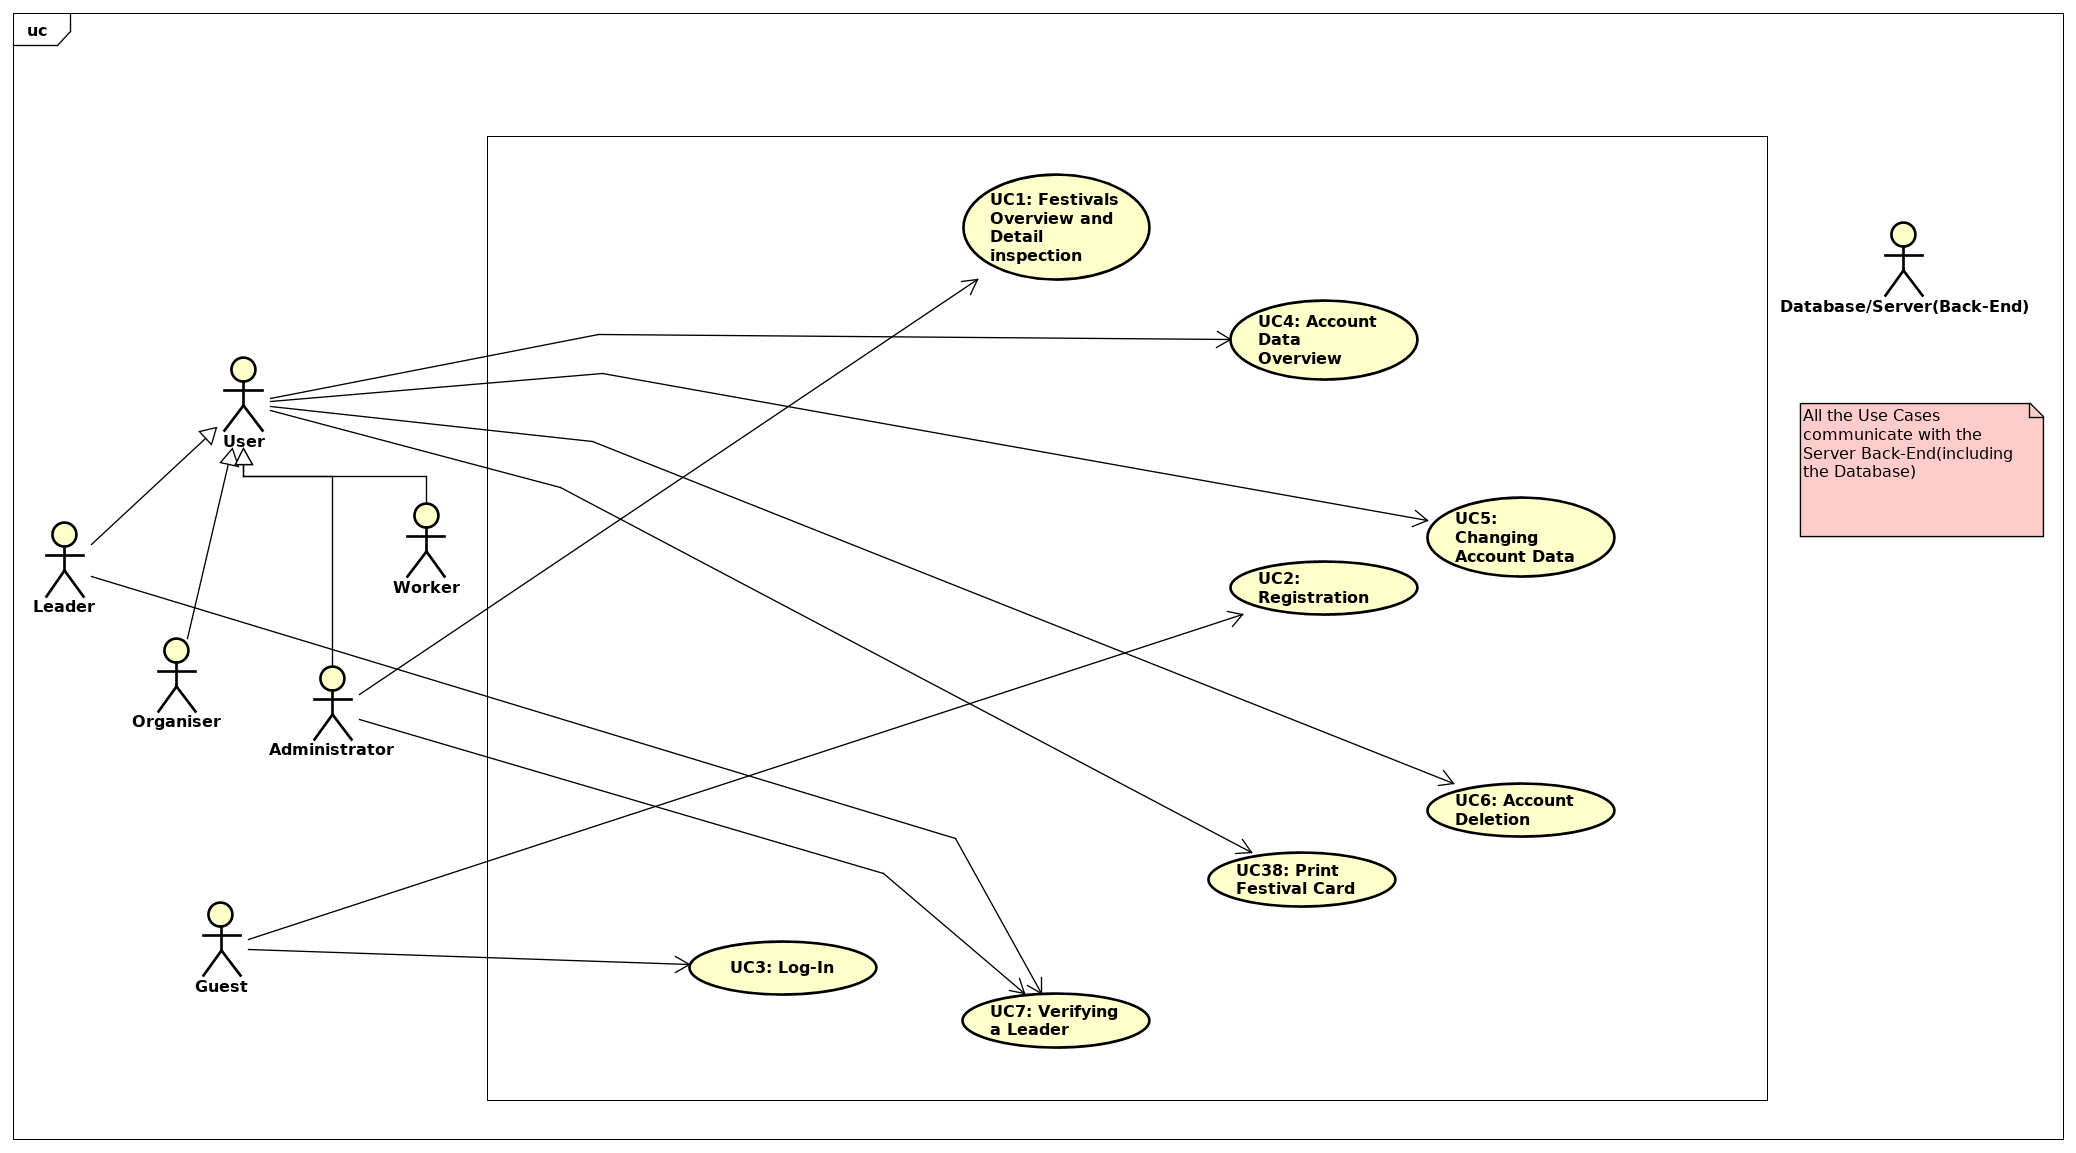
\includegraphics[width=\linewidth]{diagrams/uc-diag0-general.png}
					\caption{Use Case diagram - General Account Usage}
					\label{fig:uc_diag_0_general}
				\end{figure}
			
				\begin{figure}[H]
					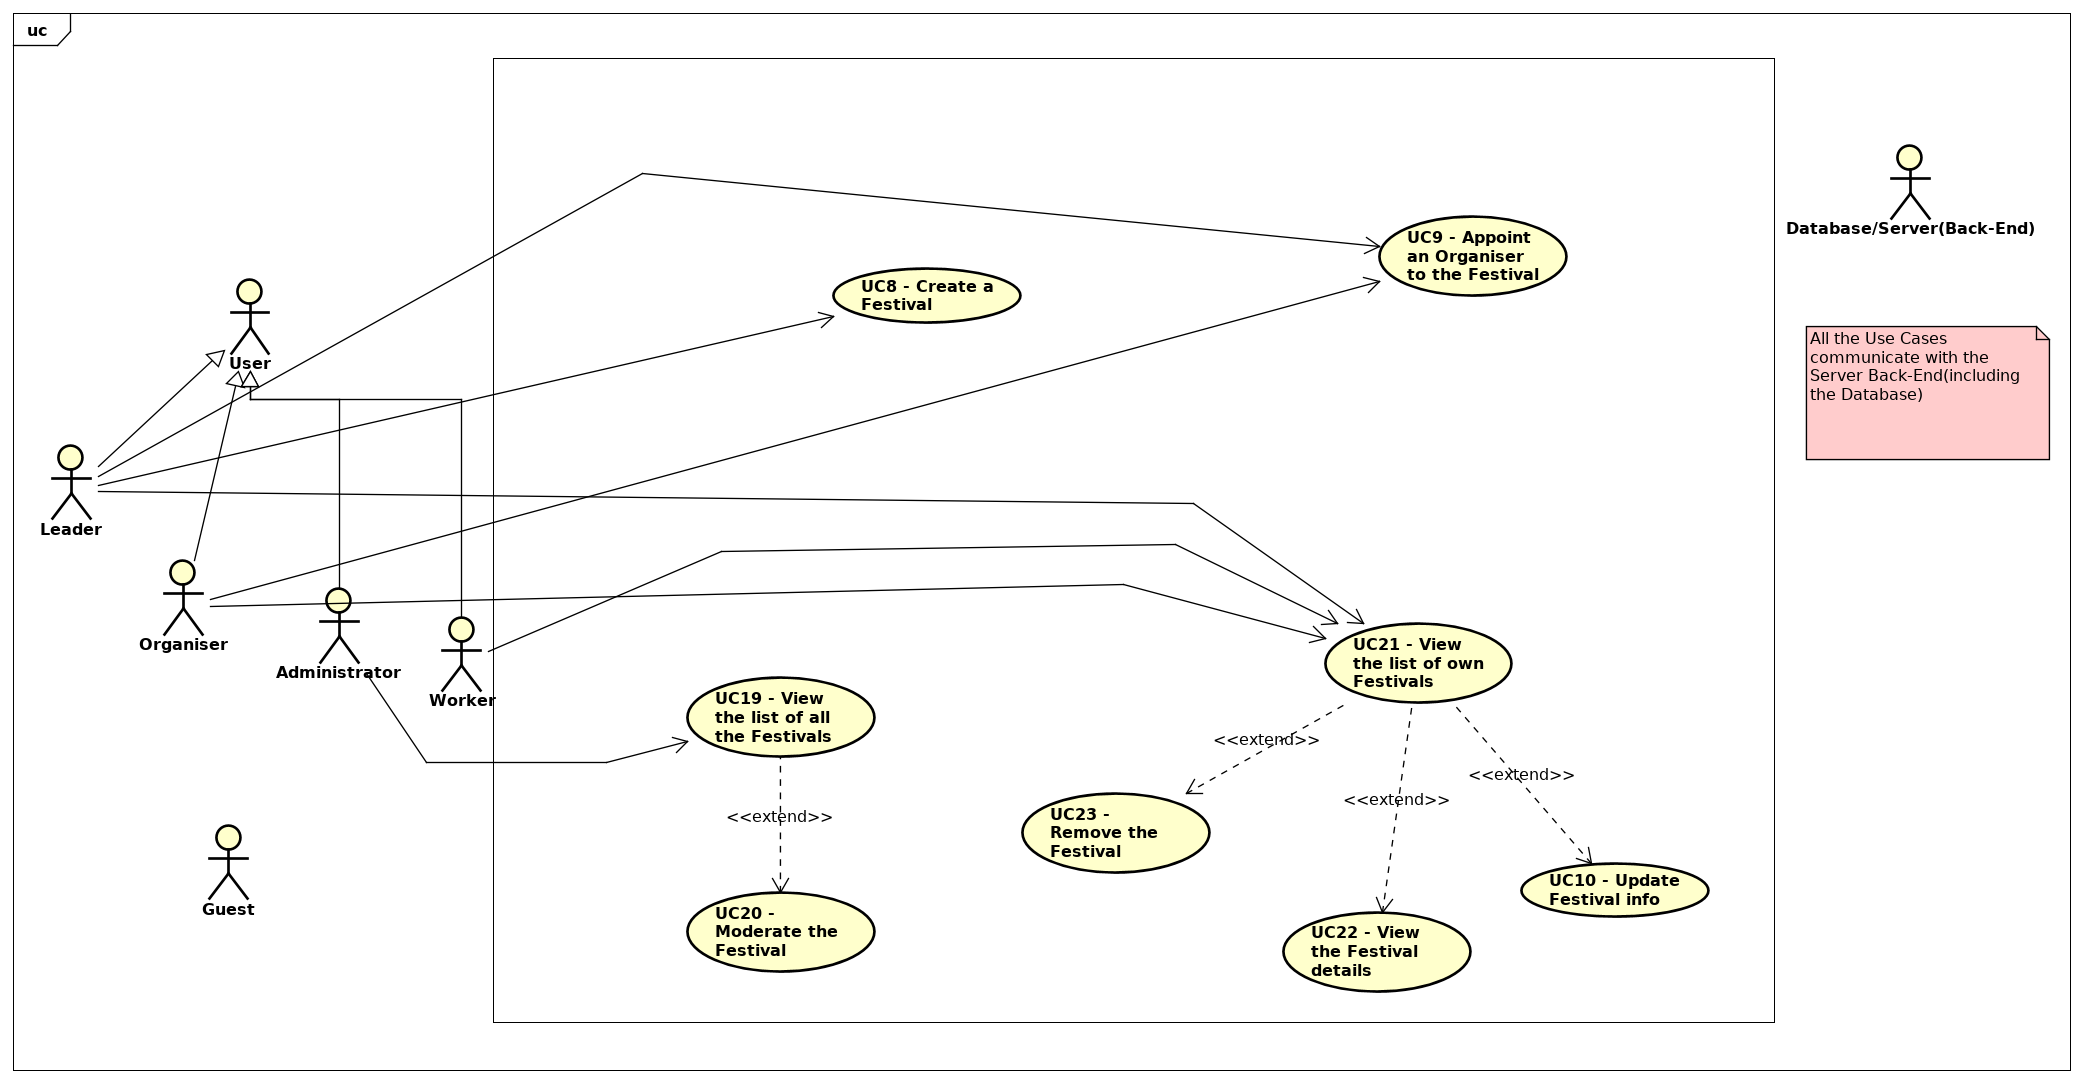
\includegraphics[width=\linewidth]{diagrams/uc-diag1-festival.png}
					\caption{Use Case diagram - Festival}
					\label{fig:uc_diag_1_festival}
				\end{figure}
		
				\begin{figure}[H]
					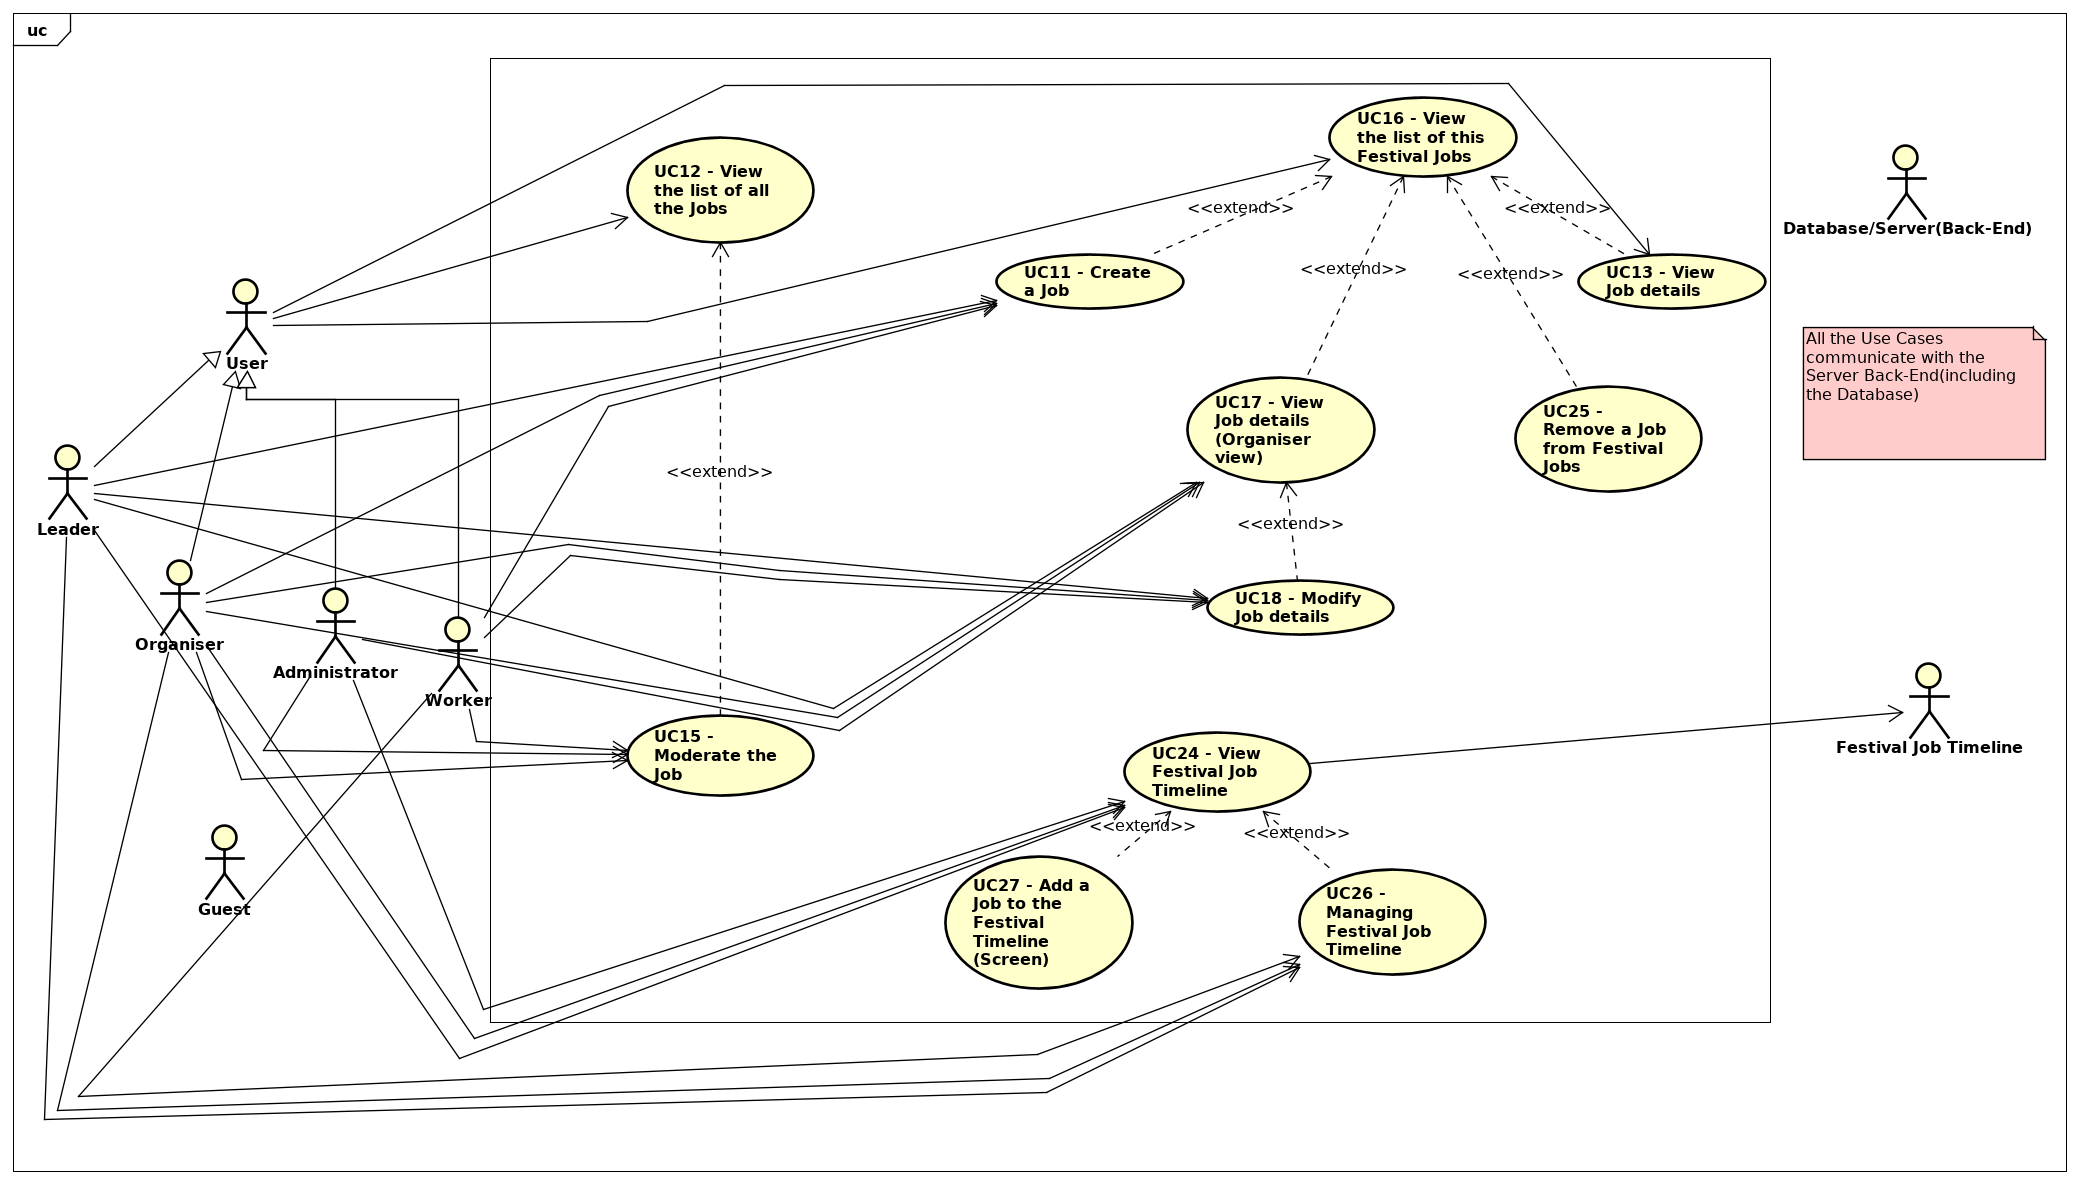
\includegraphics[width=\linewidth]{diagrams/uc-diag2-job.png}
					\caption{Use Case diagram - Job}
					\label{fig:uc_diag_2_job}
				\end{figure}
	
	
				\begin{figure}[H]
					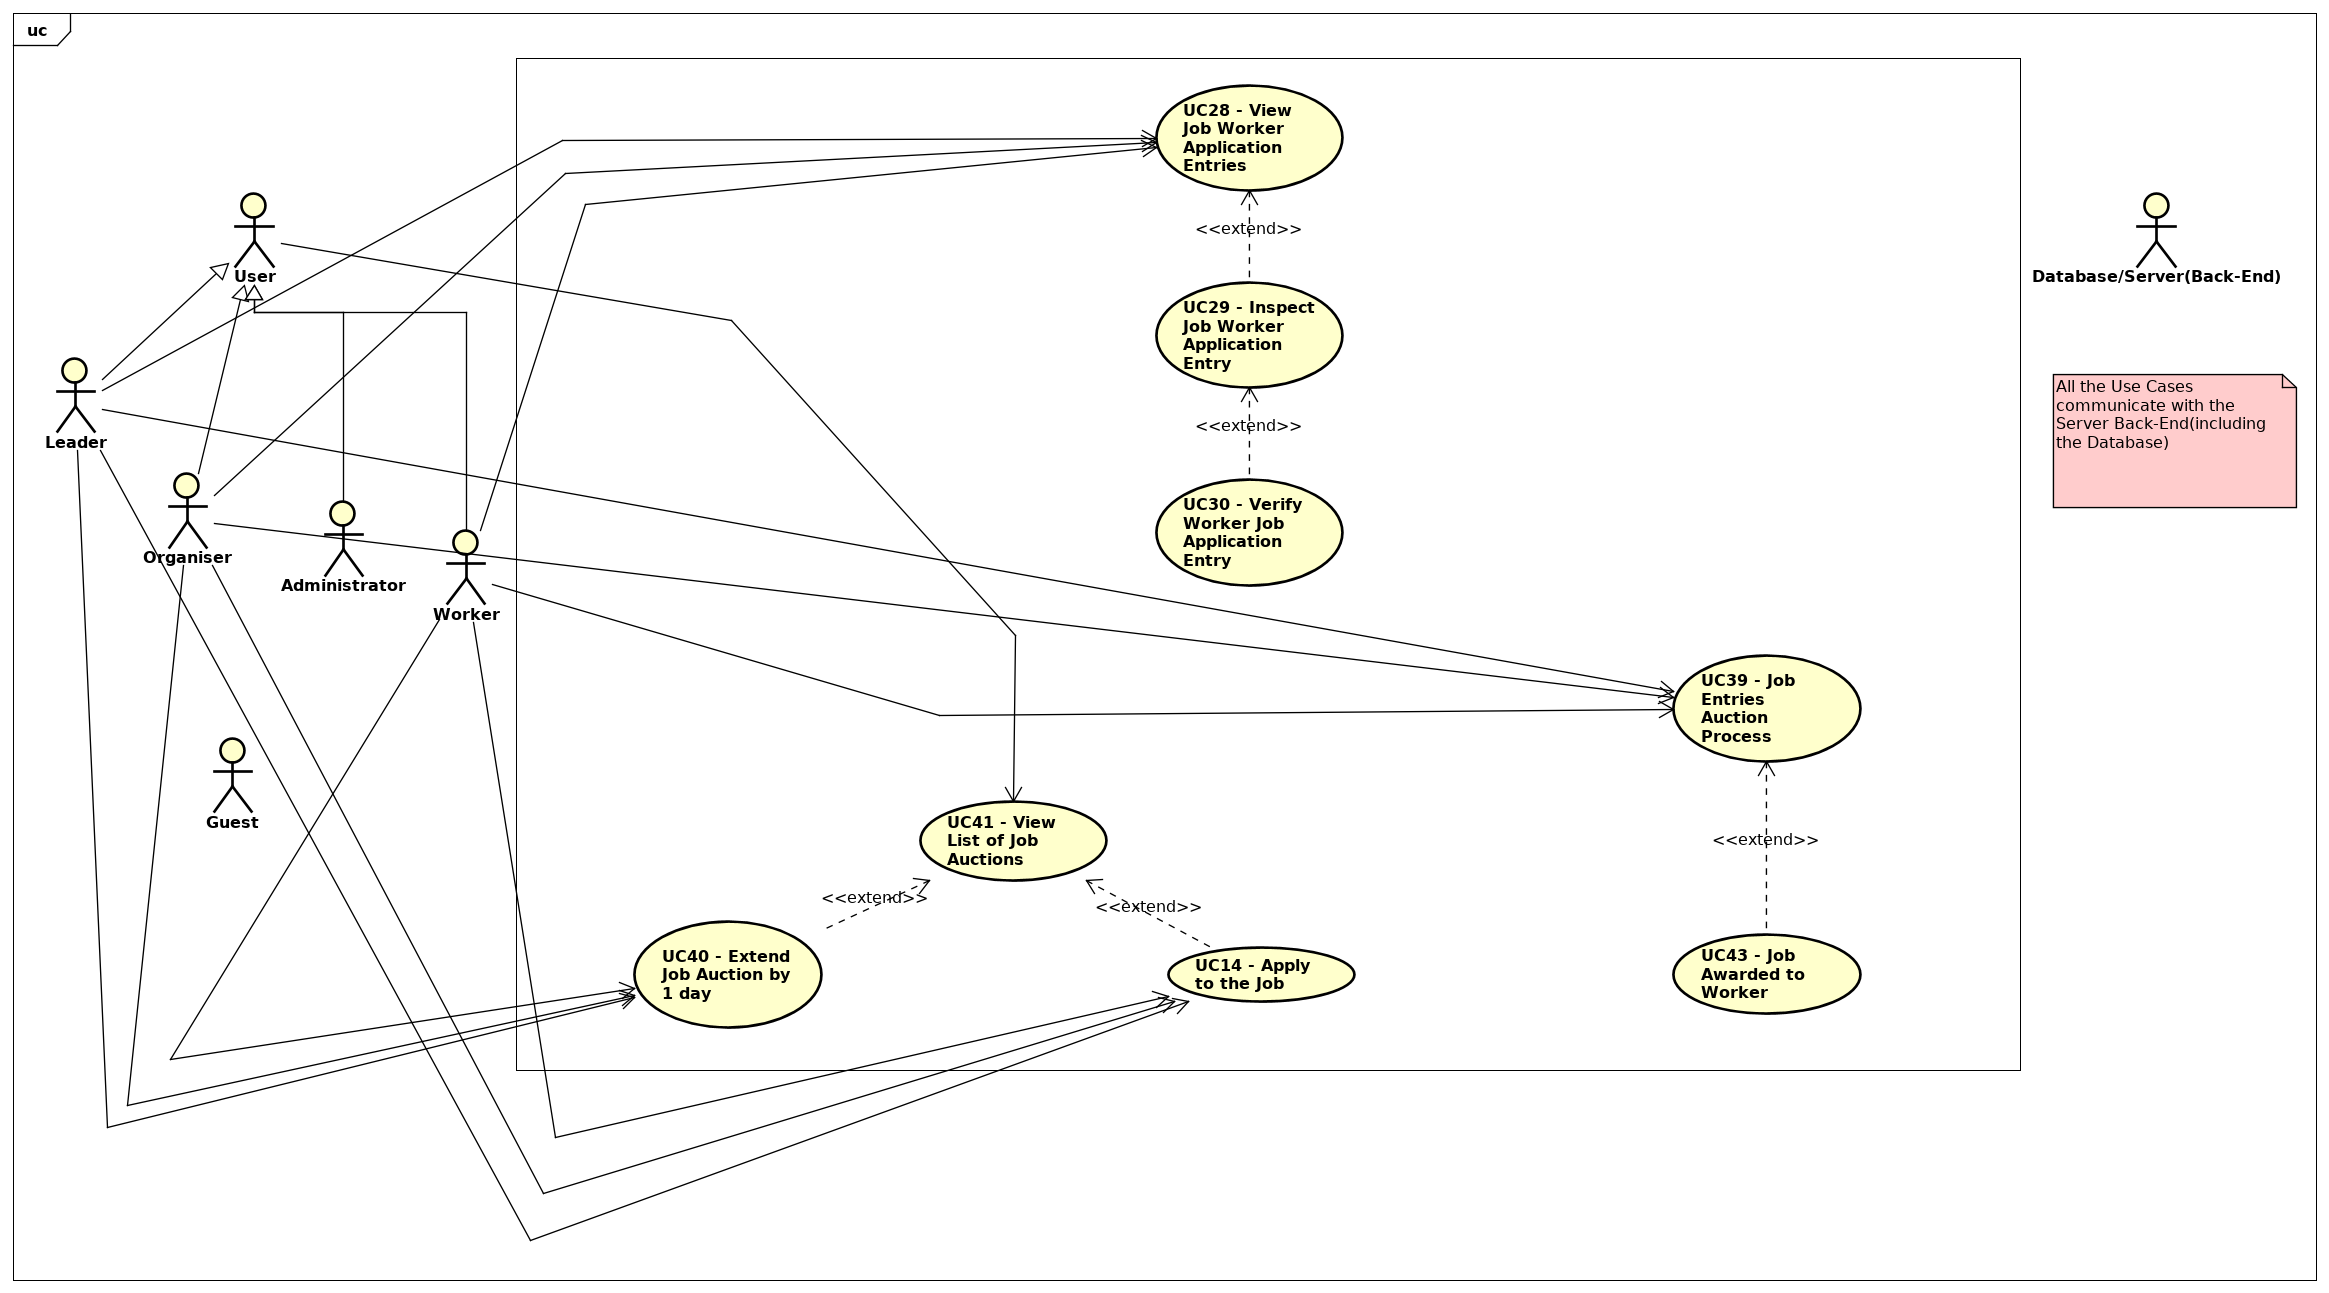
\includegraphics[width=\linewidth]{diagrams/uc-diag3-auction.png}
					\caption{Use Case diagram - Auction}
					\label{fig:uc_diag_3_auction}
				\end{figure}
			
				\begin{figure}[H]
					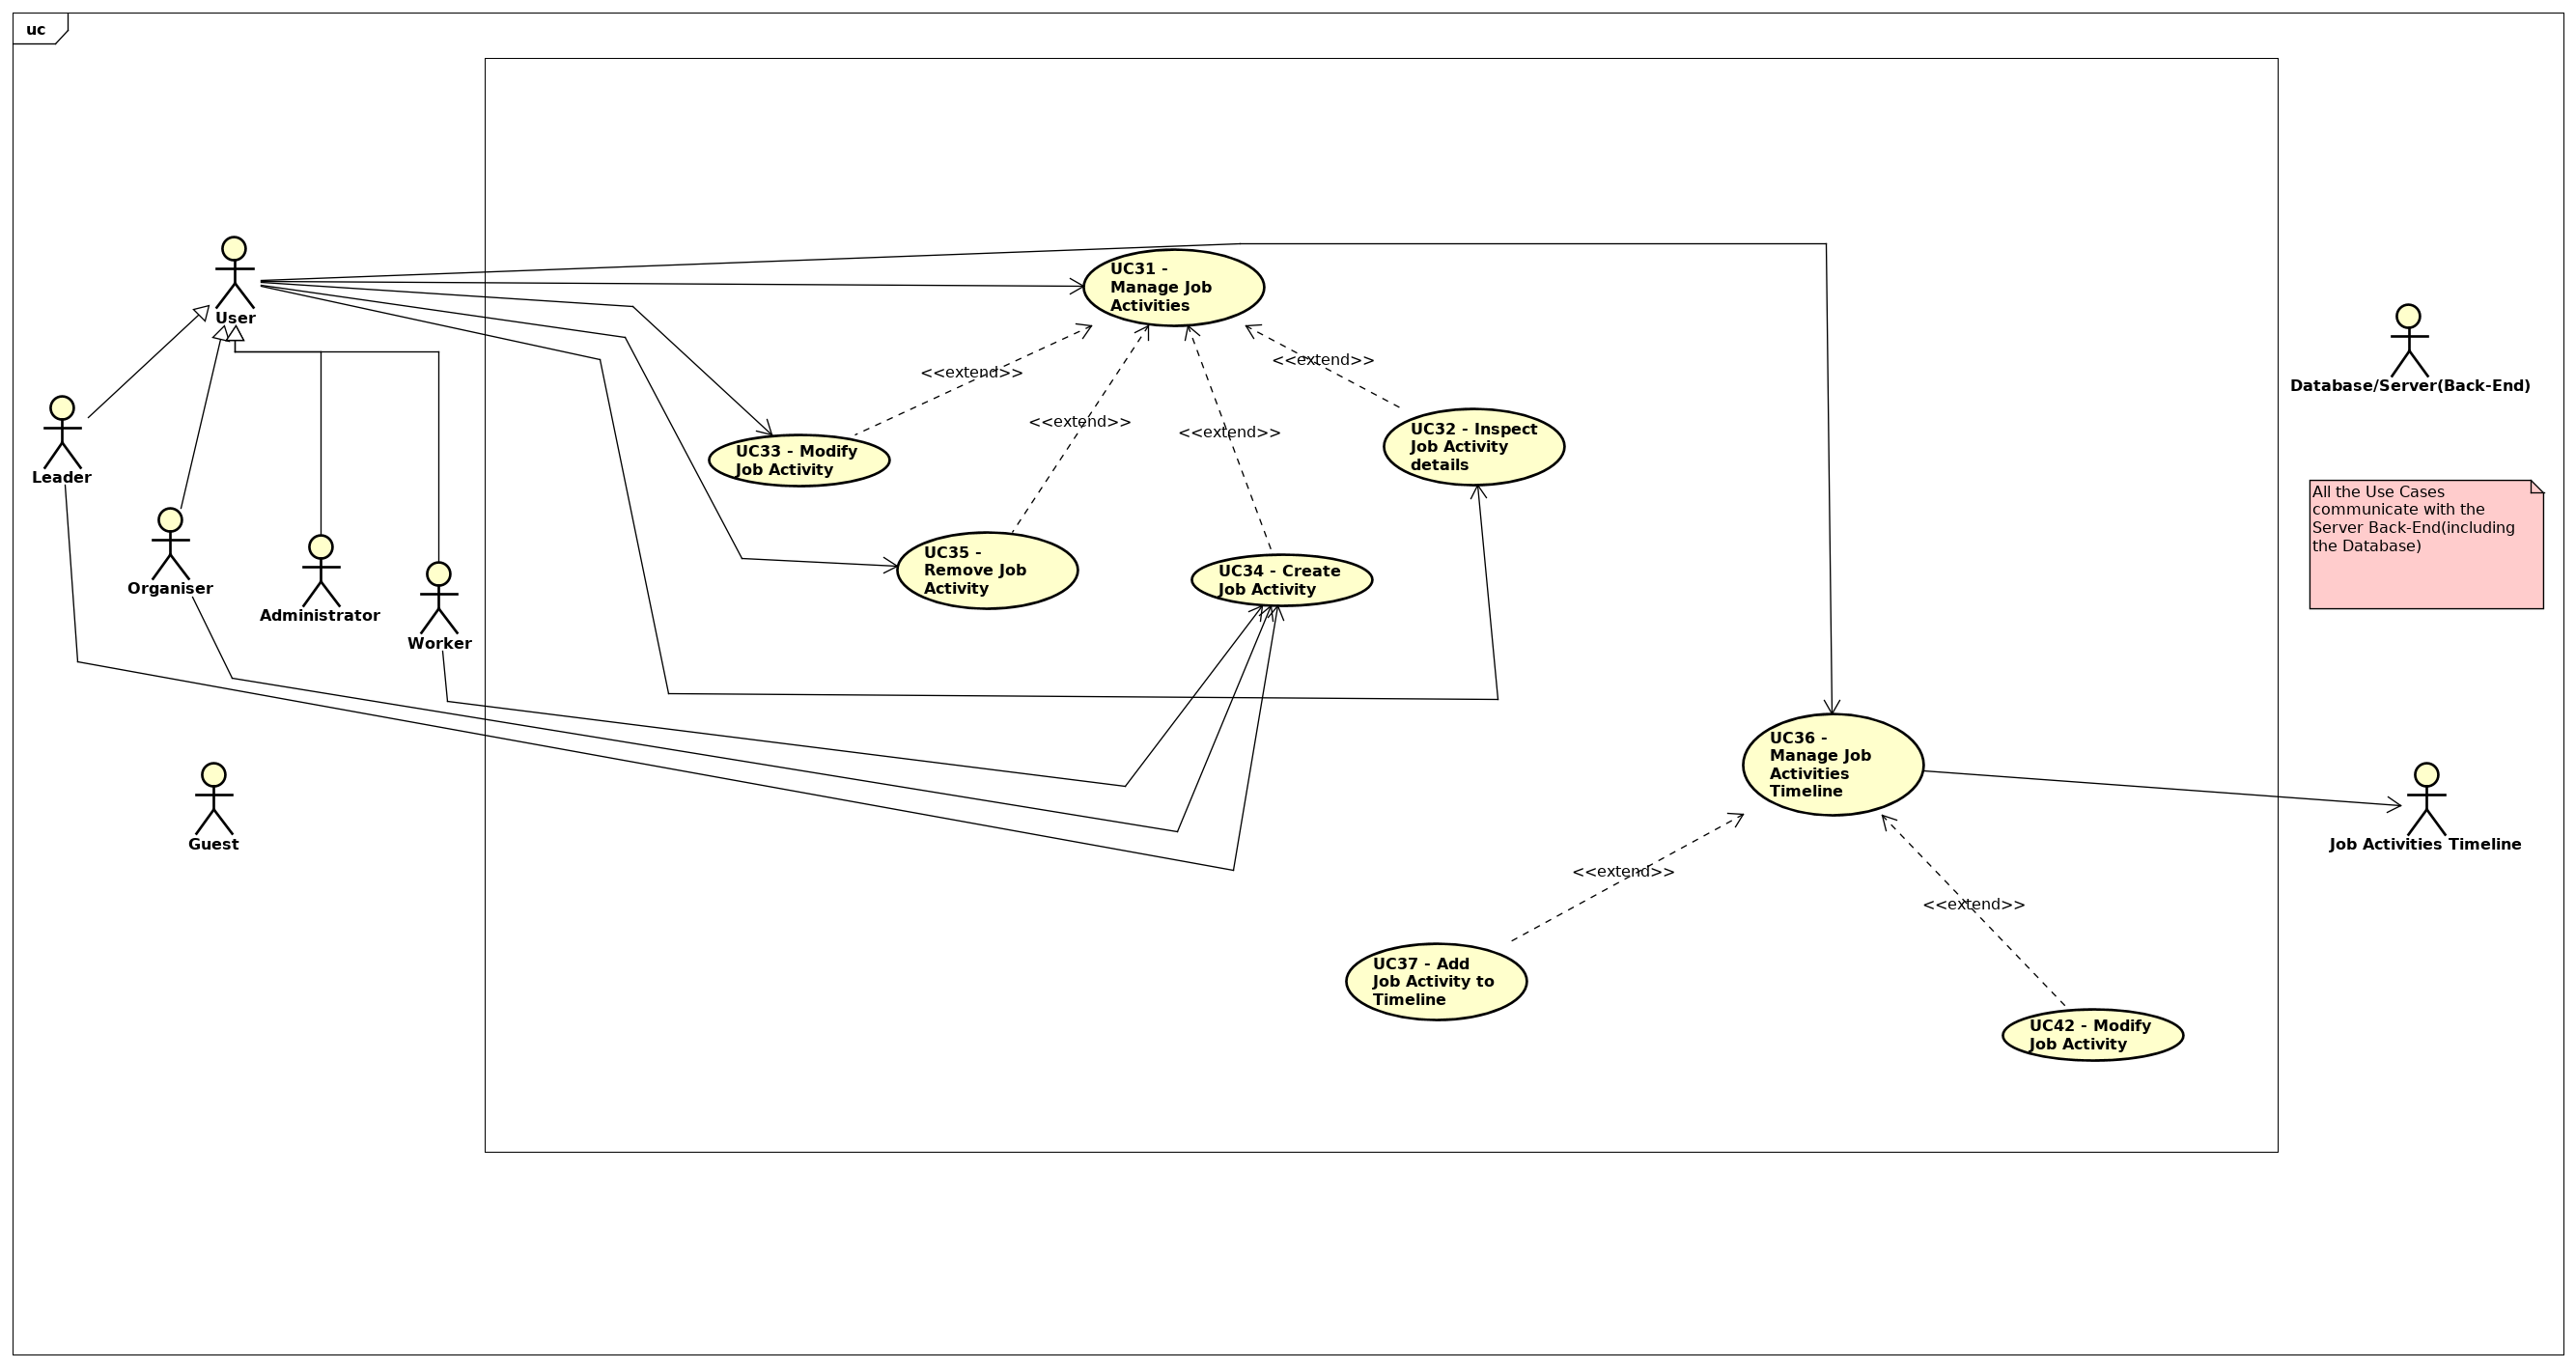
\includegraphics[width=\linewidth]{diagrams/uc-diag4-activity.png}
					\caption{Use Case diagram - Activity}
					\label{fig:uc_diag_4_activity}
				\end{figure}
				
			\subsection{Sequential Diagrams}
				
				\textbf{\textit{dio 1. revizije}}\\
				
				\textit{Nacrtati sekvencijske dijagrame koji modeliraju najvažnije dijelove sustava (max. 4 dijagrama). Ukoliko postoji nedoumica oko odabira, razjasniti s asistentom. Uz svaki dijagram napisati detaljni opis dijagrama.}
				
				\textbf{Use Case name}
				\textit{Use Case description}
				Here goes the diagram
				
				\textbf{Use Case 31 Manage Job Activities(Worker view)}
				\textit{The Worker needs to organise the Job he's been assigned. He does this by creating, modifying and removing(= manipulating) Activities that compose individual Jobs. This Use Case depicts the management of such a list of Activities that make up a Job. These Activities can then be added to the Timeline, where their time domain will be well defined and visible - this will enable an easy visualisation of the way the Job will be done and organised.}
				
				
				\eject
	
		\section{Other requirements}
		
			\textbf{\textit{dio 1. revizije}}\\
		 
			 \textit{Nefunkcionalni zahtjevi i zahtjevi domene primjene dopunjuju funkcionalne zahtjeve. Oni opisuju \textbf{kako se sustav treba ponašati} i koja \textbf{ograničenja} treba poštivati (performanse, korisničko iskustvo, pouzdanost, standardi kvalitete, sigurnost...). Primjeri takvih zahtjeva u Vašem projektu mogu biti: podržani jezici korisničkog sučelja, vrijeme odziva, najveći mogući podržani broj korisnika, podržane web/mobilne platforme, razina zaštite (protokoli komunikacije, kriptiranje...)... Svaki takav zahtjev potrebno je navesti u jednoj ili dvije rečenice.}
			 
			 \begin{packed_item}
			 	\item The System should allow concurrent usage by multiple Users
			 	\item The System should use UTF-8 - allow diacritical characters
			 	\item The System should use HRK and EUR as currency
			 	\item The System should be fast, reponsive and stable
			 	\item In case of some instability or error, the System should be able to recover gracefully and allow further usage
			 	\item User data should be stored safely and securely, as well as be accordingly encrypted
			 	\item The connection to the Server/Database should be reliable and secure
			 	\item The system should be easy and intuitive to use - not too complicated
			 	\item Implementation - using moder Object-Oriented Programming Languages such as Java or Kotlin
			 	\item The System should be as bug resistant as possible
			 \end{packed_item}
			 
			 
			 
	